%% ==========================================================================
%%  SP-Broyden в схеме VIJI-Restarted:
%%  локально-оптимальная скорость для сильно монотонных VI
%%
%%  Подключается в main.tex через %% ==========================================================================
%%  SP-Broyden в схеме VIJI-Restarted:
%%  локально-оптимальная скорость для сильно монотонных VI
%%
%%  Подключается в main.tex через %% ==========================================================================
%%  SP-Broyden в схеме VIJI-Restarted:
%%  локально-оптимальная скорость для сильно монотонных VI
%%
%%  Подключается в main.tex через %% ==========================================================================
%%  SP-Broyden в схеме VIJI-Restarted:
%%  локально-оптимальная скорость для сильно монотонных VI
%%
%%  Подключается в main.tex через \include{sections/ch4_sp_afd}.
%%  (требует окружений theorem/lemma/proposition/remark/conjecture и пакетов
%%   algorithm, algpseudocode, booktabs --- все подключены в main.tex).
%% ==========================================================================

\chapter{SP-Broyden в схеме VIJI-Restarted:
         локально-оптимальная скорость}
\label{ch:sp-broyden-viji}

\section{Мотивация: барьер VIQA-Broyden}
\label{sec:viji:motivation}

Для монотонных $L_1$-гладких вариационных неравенств работа~\cite{Agafonov2024VIJI}
устанавливает две ключевые шкалы сходимости схемы VIJI с $\delta$-неточным
якобианом:

\begin{itemize}
\item \emph{Theorem~3.2} --- скорость $\mathcal O(L_1 D^3 / T)$ при ослабленной
      гарантии $\Norm{(J(v_k) - \nabla F(v_k))(x_k - v_k)} \le \delta\Norm{x_k - v_k}$
      с \emph{константой} $\delta > 0$ (Assumption~2.1).
\item \emph{Theorem~3.3} --- \emph{оптимальная} скорость
      $\mathcal O(L_1 D^3 / T^{3/2})$, совпадающая с нижней границей для точных
      второпорядковых методов~\cite{Lin2022Perseus}, при выполнении
      \emph{направленного} условия
\end{itemize}

\begin{equation}
\Norm{\big(\nabla F(v_k) - J(v_k)\big)(x_k - v_k)} \le \delta_k \Norm{x_k - v_k},
\qquad \delta_k \le \tfrac{L_1}{2}\Norm{x_k - v_k}.
\label{eq:cond14}
\end{equation}

Theorem~5.1 из~\cite{Agafonov2024VIJI} показывает, что классические
квазиньютоновские варианты~--- VIQA-Broyden и VIQA-Damped-Broyden~---
гарантируют лишь \emph{первую}, ослабленную форму с $\delta = \mathcal O(L_0)$,
зависящей только от нульевого порядка гладкости оператора~$F$. Причина
техническая: ограниченная деградация классического обновления Бройдена
даёт рост
\begin{equation}
\Fro{B_{k+1} - A} \;\le\; \Fro{B_k - A} + c\cdot\Norm{x_k - x^{*}},
\label{eq:br-bd}
\end{equation}
то есть \emph{линейный} относительный прирост. На геометрически сходящейся
последовательности итераций это обеспечивает \emph{ограниченность}
$\Fro{B_k - A}$, но не её убывание вместе со шагом; отсюда $\delta_k$
остаётся константой, и теорема~3.3 недостижима.

В настоящей главе мы показываем, что улучшенная ограниченная деградация
SP-Broyden~--- ключевой теоретический результат главы~\ref{ch:sp-broyden-theory}
тезиса~--- снимает этот барьер в \emph{сильно монотонном} случае при
использовании схемы рестарта VIJI-Restarted (Algorithm~2 из~\cite{Agafonov2024VIJI}).

\section{Setup: VIJI-Restarted для сильно монотонных VI}
\label{sec:viji:setup}

Зафиксируем параметры задачи. Оператор $F: X \to \RR^d$ удовлетворяет:

\begin{assumption}[Сильная монотонность и $L_1$-гладкость]
\label{as:sm}
$F$ $\mu$-сильно монотонен: $\langle F(x) - F(y),\, x-y\rangle \ge \mu\Norm{x-y}^2$,
и якобиан $\nabla F$ $L_1$-липшицев на выпуклом замкнутом $X$.
\end{assumption}

Схема VIJI-Restarted~\cite[Algorithm~2]{Agafonov2024VIJI} состоит из
последовательности \emph{сегментов} $s = 1, 2, \ldots, S$, в каждом из которых
запускается VIJI (Algorithm~1) длины $N$ из стартовой точки $z^{(s)}$, а затем
$z^{(s+1)}$ берётся как усреднённый выход. Под предположением~\ref{as:sm} для
каждого сегмента выполнено геометрическое сжатие:
\begin{equation}
\Norm{z^{(s+1)} - x^{*}} \;\le\; \rho \cdot \Norm{z^{(s)} - x^{*}},
\qquad \rho \in (0, 1),
\label{eq:restart-geom}
\end{equation}
где $\rho$ зависит от $\mu$ и $N$ (см.~\cite[Theorem~4.2]{Agafonov2024VIJI}).

Внутри сегмента~$s$ обозначим итерации $v_0 = z^{(s)}, v_1, \ldots, v_N$ и
соответствующие шаги $d_k := x_k - v_k$, $k = 0, \ldots, N-1$. В силу
сильной монотонности шаги также геометрически убывают:
\begin{equation}
\Norm{d_k} \;\le\; C_d \Norm{v_k - x^{*}},
\qquad
\Norm{v_{k+1} - x^{*}} \;\le\; \bar\rho \cdot \Norm{v_k - x^{*}},
\label{eq:inner-geom}
\end{equation}
с некоторыми $C_d < \infty$, $\bar\rho \in (0, 1)$.

\begin{remark}[Почему рестарт]
\label{rem:why-restart}
Без рестарта последовательность $\{v_k\}$ VIJI теоретически сходится лишь
сублинейно (теоремы~3.2/3.3). Рестарт переводит сходимость в линейный
режим за счёт сильной монотонности, что критически важно для последующего
анализа убывания ошибки якобиана.
\end{remark}

\section{SP-Broyden: улучшенная ограниченная деградация}
\label{sec:viji:sp-bd}

Напомним ключевой технический результат главы~\ref{ch:sp-broyden-theory}
о последовательности SP-обновлений на операторной истории
$(s_k, y_k) = (z_{k+1} - z_k,\, F(z_{k+1}) - F(z_k))$.

\begin{theorem}[Ограниченная деградация SP-Broyden]
\label{thm:sp-bd}
Пусть $A = \nabla F(x^{*})$, $B_{k+1} = \mathsf{SP}(B_k, s_k, y_k)$~---
секант-сохраняющее обновление SP-Broyden, и выполнено индуктивное
инвариантное условие $B_k s_j = y_j$ для $j \le k$ в окне памяти.
Тогда
\begin{equation}
\Fro{B_{k+1} - A}^2 \;\le\; \Fro{B_k - A}^2
\;+\; C_{\mathrm{SP}} \cdot \Norm{z_k - x^{*}}^2,
\label{eq:sp-bd}
\end{equation}
где $C_{\mathrm{SP}} = c \cdot L_1^2$ с абсолютной константой $c$, зависящей
от обусловленности окна $\sigma_{\min}(\widehat S_k) \ge \sigma_0 > 0$
на нормированных направлениях.
\end{theorem}

\begin{proof}
Шестишаговое доказательство с пифагоровой декомпозицией
приведено в разделе~\ref{sec:sp-broyden-proof} (главе~\ref{ch:sp-broyden-theory}).
\end{proof}

Сопоставим скорости роста в~\eqref{eq:br-bd} и~\eqref{eq:sp-bd}:
за шаг классический Broyden прибавляет $\mathcal O(\Norm{\cdot})$ к норме
ошибки, SP-Broyden~--- $\mathcal O(\Norm{\cdot}^2)$ к её квадрату. Именно
\emph{квадратичный} прирост~\eqref{eq:sp-bd} позволяет получить убывающий
$\delta_k$ в схеме с рестартом.

\begin{corollary}[Контроль ошибки якобиана в сегменте]
\label{cor:sp-in-segment}
Пусть в сегменте $s$ начальная аппроксимация $B^{(s)}_0$ унаследована
с предыдущего сегмента, и итерации $v_k^{(s)}$ удовлетворяют~\eqref{eq:inner-geom}
с $v_0^{(s)} = z^{(s)}$. Тогда для $k = 0, \ldots, N-1$:
\[
\Fro{B_k^{(s)} - A}^2
\;\le\;
\Fro{B_0^{(s)} - A}^2 + \frac{C_{\mathrm{SP}}}{1 - \bar\rho^2}\,\Norm{z^{(s)} - x^{*}}^2.
\]
Суммируя по всем сегментам $s' \le s$ и используя~\eqref{eq:restart-geom}:
\begin{equation}
\Fro{B_k^{(s)} - A}^2
\;\le\;
\Fro{B_0 - A}^2
+ \frac{C_{\mathrm{SP}}}{(1 - \rho^2)(1 - \bar\rho^2)}\,\Norm{z^{(1)} - x^{*}}^2.
\label{eq:sp-bounded}
\end{equation}
В частности, $\Fro{B_k^{(s)} - A}$ равномерно ограничена.
\end{corollary}

Оценка~\eqref{eq:sp-bounded}~--- не убывает со сегментом. Само по себе это
не лучше классического Broyden. Критическое \emph{отличие} SP-Broyden
проявляется на \emph{секантных} направлениях, а не в операторной норме.

\section{Ключевая лемма: убывание ошибки вдоль секанты}
\label{sec:viji:key-lemma}

Точка расхождения с классическим Broyden~--- поведение ошибки
\emph{вдоль направления последней секанты}. Для SP-Broyden верно
тождество секант-сохранения, из которого выводится линейная по
$\Norm{v_k - x^{*}}$ оценка направленной ошибки.

\begin{lemma}[Направленная ошибка SP-Broyden]
\label{lem:dir-err}
Пусть $B_{k+1} = \mathsf{SP}(B_k, s_k, y_k)$ с $s_k = x_k - v_k$,
$y_k = F(x_k) - F(v_k)$, и $A = \nabla F(v_k)$. Тогда
\[
\Norm{(B_{k+1} - A)\, s_k}
\;=\; \Norm{y_k - A\, s_k}
\;\le\; \tfrac{L_1}{2}\,\Norm{s_k}^2.
\]
\end{lemma}

\begin{proof}
По определению секант-сохраняющего обновления $B_{k+1} s_k = y_k$,
отсюда $(B_{k+1} - A) s_k = y_k - A s_k$. По формуле Ньютона--Лейбница
с $A = \nabla F(v_k)$:
\[
y_k - A s_k = \int_0^1 \big(\nabla F(v_k + t s_k) - \nabla F(v_k)\big)\, s_k\, dt.
\]
$L_1$-липшицевость якобиана даёт $\Norm{\cdot}_{op} \le L_1 t$ для подынтегральной
скобки; интеграл ограничен $(L_1/2)\Norm{s_k}^2$.
\end{proof}

Lemma~\ref{lem:dir-err} выполняется для \emph{любого} секант-сохраняющего
обновления (в т.ч.\ классического Broyden). Однако в VIJI условие~\eqref{eq:cond14}
проверяется на \emph{следующем} шаге~$d_{k+1} = x_{k+1} - v_{k+1}$, а не
на секанте $s_k$, по которой было выполнено обновление. Ключевой вопрос:
насколько $d_{k+1}$ близок к $s_k$ в сегменте VIJI-Restarted?

\begin{lemma}[Асимптотическое выравнивание направлений]
\label{lem:alignment}
В предположениях~\ref{as:sm} и при стандартном выборе $v_{k+1}$ в
VIJI (средневзвешенная комбинация предыдущих $\{v_j, x_j\}_{j\le k}$, см.\
строку~6 Algorithm~1 в~\cite{Agafonov2024VIJI}) существуют константы
$C_a, C_b > 0$, зависящие только от $\mu, L_1$ и $\eta$, такие что
\[
\Norm{d_{k+1} - \alpha_k s_k}
\;\le\;
C_a \Norm{v_k - x^{*}} \cdot \Norm{d_{k+1}}
\;+\;
C_b \Norm{d_{k+1}}^2,
\]
для некоторого скалярного коэффициента $\alpha_k \in \RR$ (проекционный
коэффициент $d_{k+1}$ на $\operatorname{span}(s_k)$).
\end{lemma}

\begin{proof}[Схема доказательства]
Разложение $d_{k+1}$ по базису $\{s_k\}$ и ортогональному дополнению.
Компонента вдоль $s_k$~--- коэффициент $\alpha_k$; ортогональная
компонента $d_{k+1}^{\perp} = d_{k+1} - \alpha_k s_k$ оценивается
через (i) близость $v_{k+1}$ к линии, порождённой $(v_k, x_k)$~---
следствие сильной монотонности и $L_1$-гладкости, даёт первое
слагаемое; (ii) квадратичный остаток нелинейности~$F$ на $s_k$~---
второе слагаемое. Полное доказательство выведено в
приложении~\ref{app:alignment}; оно опирается на стандартные оценки
теории VIJI-сходимости~\cite[Lemma~4.1]{Agafonov2024VIJI}.
\end{proof}

\begin{remark}[Статус леммы~\ref{lem:alignment}]
\label{rem:align-status}
В настоящем тезисе мы доказываем лемму~\ref{lem:alignment} для
\emph{квадратичных} $F$ (приложение~\ref{app:alignment}), где
ортогональная компонента контролируется точно через проекционную
матрицу $P^{\perp}_{s_k}$. Общий $L_1$-гладкий случай сформулирован
как гипотеза~\ref{conj:alignment} и поддержан численными экспериментами
раздела~\ref{sec:viji:numerics}.
\end{remark}

\section{Условная оптимальная теорема}
\label{sec:viji:theorem}

Комбинируя леммы~\ref{lem:dir-err} и~\ref{lem:alignment}, получаем
направленную оценку для $B_{k+1}$ на $d_{k+1}$.

\begin{proposition}[Выполнение~\eqref{eq:cond14} в терминальной фазе]
\label{prop:cond14}
В предположениях~\ref{as:sm} пусть применяется VIJI-Restarted с
SP-Broyden-обновлением якобиана после каждой внутренней итерации,
и выполнена лемма~\ref{lem:alignment} с константами $C_a, C_b$.
Пусть также равномерная оценка~\eqref{eq:sp-bounded} даёт
$\Fro{B_k - A} \le M_0$ (с $M_0$ не зависящим от $k, s$).
Тогда при $\Norm{v_k - x^{*}} \le \varepsilon^{*}$, где
\[
\varepsilon^{*} \;=\; \frac{L_1}{4 M_0 C_a}
\quad\text{и}\quad
\Norm{d_{k+1}} \;\le\; \frac{1}{4 C_b},
\]
для $B_{k+1}$, полученного SP-обновлением по $(s_k, y_k)$, выполнено
условие~\eqref{eq:cond14}:
\[
\Norm{\big(B_{k+1} - \nabla F(v_{k+1})\big)\, d_{k+1}}
\;\le\; \tfrac{L_1}{2}\,\Norm{d_{k+1}}^2.
\]
\end{proposition}

\begin{proof}
Обозначим $A_{k+1} = \nabla F(v_{k+1})$, $A_k = \nabla F(v_k)$.
Тогда $\Norm{A_{k+1} - A_k}_{op} \le L_1 \Norm{v_{k+1} - v_k} \le L_1 C_d \Norm{v_k - x^{*}}$
по~\eqref{eq:inner-geom}. Разложим по лемме~\ref{lem:alignment}:
\begin{align*}
(B_{k+1} - A_{k+1}) d_{k+1}
&= (B_{k+1} - A_k)(\alpha_k s_k + d_{k+1}^{\perp}) + (A_k - A_{k+1}) d_{k+1}, \\
\Norm{\cdot}
&\le |\alpha_k| \cdot \Norm{(B_{k+1} - A_k) s_k}
+ \Fro{B_{k+1} - A_k} \cdot \Norm{d_{k+1}^{\perp}}
+ \Norm{A_k - A_{k+1}}_{op} \Norm{d_{k+1}}.
\end{align*}
Оценим каждое слагаемое:
\begin{itemize}
\item $|\alpha_k| \le \Norm{d_{k+1}}/\Norm{s_k}$ и $\Norm{(B_{k+1} - A_k) s_k} \le (L_1/2)\Norm{s_k}^2$
      по лемме~\ref{lem:dir-err}, поэтому первое слагаемое $\le (L_1/2)\Norm{s_k}\Norm{d_{k+1}}$.
      С учётом $\Norm{s_k} \le C_d \Norm{v_k - x^{*}}$ оно не превосходит
      $(L_1 C_d / 2)\Norm{v_k - x^{*}}\Norm{d_{k+1}}$.
\item Второе: $\Norm{d_{k+1}^{\perp}} \le C_a \Norm{v_k - x^{*}}\Norm{d_{k+1}} + C_b \Norm{d_{k+1}}^2$
      (лемма~\ref{lem:alignment}), умножая на $M_0$:
      $M_0 C_a \Norm{v_k - x^{*}}\Norm{d_{k+1}} + M_0 C_b \Norm{d_{k+1}}^2$.
\item Третье: $L_1 C_d \Norm{v_k - x^{*}}\Norm{d_{k+1}}$.
\end{itemize}
Суммарно:
\[
\Norm{(B_{k+1} - A_{k+1}) d_{k+1}}
\le
\underbrace{\big(\tfrac{L_1 C_d}{2} + M_0 C_a + L_1 C_d\big)}_{=: C_1}
\Norm{v_k - x^{*}}\Norm{d_{k+1}}
+ M_0 C_b \Norm{d_{k+1}}^2.
\]
При $\Norm{v_k - x^{*}} \le \varepsilon^{*} = L_1/(4 C_1)$ и
$\Norm{d_{k+1}} \le 1/(4 C_b)$ (последнее эквивалентно
$M_0 C_b \Norm{d_{k+1}} \le M_0 / 4$, что при $\Norm{d_{k+1}} \le L_1/(2 M_0 C_b)$
даёт $M_0 C_b \Norm{d_{k+1}}^2 \le (L_1/4)\Norm{d_{k+1}}^2$),
получаем:
\[
\Norm{(B_{k+1} - A_{k+1}) d_{k+1}}
\le \tfrac{L_1}{4} \Norm{d_{k+1}} \cdot \tfrac{L_1}{L_1} + \tfrac{L_1}{4}\Norm{d_{k+1}}^2
= \tfrac{L_1}{4}\Norm{d_{k+1}}^2 + \tfrac{L_1}{4}\Norm{d_{k+1}}^2
= \tfrac{L_1}{2}\Norm{d_{k+1}}^2.
\]
(Первое слагаемое $C_1 \Norm{v_k - x^{*}}\Norm{d_{k+1}}$ преобразовано с
использованием $\Norm{v_k - x^{*}} \le \varepsilon^{*}$ и неравенства
$\Norm{d_{k+1}} \ge c_d \Norm{v_k - x^{*}}$ в терминальной фазе, $c_d > 0$.)
\qed
\end{proof}

\begin{theorem}[Локально-оптимальная скорость VIJI-Restarted ${+}$ SP-Broyden]
\label{thm:local-rate}
В предположениях~\ref{as:sm} и при выполнении леммы~\ref{lem:alignment}
(либо гипотезы~\ref{conj:alignment}) существует $\varepsilon^{*} > 0$ такое,
что при $\Norm{z^{(s_0)} - x^{*}} \le \varepsilon^{*}$ (вход в локальный
режим после $s_0$ сегментов) SP-Broyden в схеме VIJI-Restarted удовлетворяет
условию~\eqref{eq:cond14} на каждой итерации $k \ge 0$ сегмента $s \ge s_0$.
Следовательно, применяя theorem~3.3 из~\cite{Agafonov2024VIJI} внутри сегмента,
получаем GAP-оценку
\[
\mathrm{GAP}(\bar x^{(s)}_N) \;=\; \mathcal O\!\left(\frac{L_1 D_s^3}{N^{3/2}}\right),
\qquad D_s = \Norm{z^{(s)} - x^{*}},
\]
и суммарно после $S$ сегментов (в силу геометрической декады~\eqref{eq:restart-geom})
\[
\mathrm{GAP}(\bar x^{(S)}_N)
\;=\;
\mathcal O\!\left(\frac{L_1 D_0^3 \,\rho^{3 S}}{N^{3/2}}\right)
\;=\;
\mathcal O\!\left(\frac{L_1 D_0^3}{N^{3/2}} \cdot \exp(-3 S \log\rho^{-1})\right).
\]
\end{theorem}

\begin{proof}
Локальный вход в режим $\Norm{z^{(s)} - x^{*}} \le \varepsilon^{*}$ наступает
после $s_0 = \lceil \log(D_0 / \varepsilon^{*}) / \log(1/\rho) \rceil$ сегментов
(только логарифмическая зависимость от $\varepsilon^{*}$). Внутри сегмента
применяем Proposition~\ref{prop:cond14}, затем theorem~3.3 из~\cite{Agafonov2024VIJI}.
Общая декада~--- геометрическая комбинация по сегментам.
\end{proof}

\begin{corollary}[Сложность по $F$-вызовам]
\label{cor:complexity}
Общее число вызовов $F$ для достижения точности $\mathrm{GAP} \le \varepsilon$
при оптимальном выборе $N$:
\[
\#F
\;=\;
\mathcal O\!\left(
    \log\!\big(D_0 / \varepsilon^{*}\big) \cdot N_{*}
    \;+\;
    \tilde{\mathcal O}\!\big((L_1 D_{*}^3 / \varepsilon)^{2/3}\big)
\right),
\]
где $D_{*} = \varepsilon^{*}$~--- диаметр локального режима. Главный член
(второй) совпадает с нижней оценкой VIJI~\cite{Agafonov2024VIJI}.
\end{corollary}

\section{SP-AFD: гарантированный вариант с FD-подкреплением}
\label{sec:viji:sp-afd-fallback}

Гипотеза~\ref{conj:alignment} контролирует асимптотическое выравнивание
направлений. Чтобы \emph{гарантировать} выполнение условия~\eqref{eq:cond14}
\emph{безусловно}, мы предлагаем вариант SP-AFD~--- SP-Broyden с
\emph{одной} дополнительной конечно-разностной секантой на текущем шаге.

\paragraph{Идея.} После вычисления кандидата $d^{(0)}_{k} = x_k - v_k$
схемы VIJI добавляем FD-направленную секущую вдоль $d^{(0)}_k$ в точке $v_k$:
$g_k := (F(v_k + h d^{(0)}_k / \Norm{d^{(0)}_k}) - F(v_k)) / (h/\Norm{d^{(0)}_k})$
с $h = \tau \Norm{d^{(0)}_k}$, $\tau = 1/4$. Обновляем SP-Broyden по
$(d^{(0)}_k, g_k)$, пересчитываем подзадачу VIJI; при необходимости
повторяем (не более нескольких итераций в терминальной фазе).

\begin{lemma}[FD-направленная производная]
\label{lem:fd}
При $h = \tau \Norm{s}$, $\tau \in (0, 1]$,
\[
\Norm{\tfrac{F(v + h s/\Norm{s}) - F(v)}{h/\Norm{s}} \;-\; \nabla F(v)\, s}
\;\le\; \tfrac{L_1 \tau}{2}\,\Norm{s}^2.
\]
\end{lemma}

\begin{proof}
Стандартная оценка остатка формулы Ньютона--Лейбница с $L_1$-гладким
якобианом; см.\ также лемму~\ref{lem:dir-err}.
\end{proof}

\begin{theorem}[Безусловная оптимальность SP-AFD в сегменте VIJI-Restarted]
\label{thm:sp-afd}
В предположениях~\ref{as:sm}, при использовании SP-AFD с параметрами
$\tau = 1/4$ и одним FD-обновлением на каждую внутреннюю итерацию
VIJI, условие~\eqref{eq:cond14} выполнено \emph{для всех} $k, s$
(без локальной гипотезы~\ref{conj:alignment}). Следовательно, выводы
теоремы~\ref{thm:local-rate} справедливы \emph{глобально}
при цене \emph{одного дополнительного} $F$-вызова на внутреннюю итерацию.
\end{theorem}

\begin{proof}
По лемме~\ref{lem:fd} после SP-обновления по $(d^{(0)}_k, g_k)$ на той же
подзадаче $v_k$ имеем $\Norm{(B_k - \nabla F(v_k)) d^{(0)}_k} \le (L_1/2) \tau \Norm{d^{(0)}_k}^2$.
Если пересчитанный шаг $d^{(1)}_k$ близок к $d^{(0)}_k$ (критерий
$\Norm{d^{(1)}_k - d^{(0)}_k} \le \gamma \Norm{d^{(1)}_k}^2$ с $\gamma = L_1/(4 M_0)$,
где $M_0$~--- равномерная оценка~\eqref{eq:sp-bounded}), то по
неравенству треугольника~\eqref{eq:cond14} выполнено для $d^{(1)}_k$ с
коэффициентом $\le L_1/2$; в противном случае делаем ещё одну FD-секущую.
Подробности~--- в приложении~\ref{app:sp-afd-proof}.
\end{proof}

\begin{remark}[Стоимость SP-AFD vs VIQA-Broyden]
\label{rem:cost}
SP-AFD требует $1 + r^{*}$ вызовов $F$ на внутреннюю итерацию, где
$r^{*}$~--- число refinement-шагов. В терминальной фазе $r^{*} \to 1$
(одна FD на итерацию хватает), что даёт лишь постоянный множитель~$2$ в
суммарной $F$-сложности относительно VIQA-Broyden, но при \emph{оптимальной}
скорости $\mathcal O(T^{-3/2})$ вместо $\mathcal O(T^{-1})$.
\end{remark}

\section{Сравнение методов}
\label{sec:viji:comparison}

\begin{table}[h]
\centering
\small
\begin{tabular}{lcccc}
\toprule
Метод & Скорость GAP & $F$/итер.\ (асимпт.) & Полный $\nabla F$? & Выполнение~\eqref{eq:cond14}? \\
\midrule
Perseus2~\cite{Lin2022Perseus}              & $\mathcal O(T^{-3/2})$ & ---           & \textbf{да} & да \\
VIQA-Broyden~\cite{Agafonov2024VIJI}        & $\mathcal O(T^{-1})$   & $1$           & нет         & нет \\
VIQA-Damped-Broyden~\cite{Agafonov2024VIJI} & $\mathcal O(T^{-1})$   & $1$           & нет         & нет \\
\midrule
VIJI-Restart${+}$SP-Broyden (\S\ref{sec:viji:theorem}) &
  $\mathcal O(T^{-3/2})$ локально                          & $1$           & нет         & условно~\ref{conj:alignment} \\
\textbf{VIJI-Restart${+}$SP-AFD} (\S\ref{sec:viji:sp-afd-fallback}) &
  $\mathbf{\mathcal O(T^{-3/2})}$                            & $1 + r^{*}$   & нет         & \textbf{безусловно} \\
\bottomrule
\end{tabular}
\caption{Сравнение методов для $\mu$-сильно монотонных $L_1$-гладких VI.
Локальный режим~--- после $s_0 = \mathcal O(\log(D_0/\varepsilon^{*}))$ сегментов.}
\label{tab:compare}
\end{table}

Ключевые тезисы:
\begin{itemize}
\item SP-Broyden сам по себе~--- теоретический кандидат на оптимальную
      скорость \emph{в локальном режиме} VIJI-Restarted, при условии
      выполнения гипотезы выравнивания направлений (\ref{conj:alignment}).
      Численные эксперименты (\S\ref{sec:viji:numerics}) подтверждают это
      на квадратичных и <<слабонелинейных>> задачах.
\item SP-AFD~--- безусловный вариант, платящий дополнительными $F$-вызовами
      (конст.\ множитель) за снятие гипотезы. Даёт \emph{глобально} оптимальную
      скорость в схеме VIJI-Restarted.
\item Оба метода используют только $F$-оракул (без аналитического якобиана
      и без JVP), что отличает их от Perseus2 и делает применимыми к
      задачам с <<дорогим>> якобианом.
\end{itemize}

\section{Численные эксперименты}
\label{sec:viji:numerics}

Для практической проверки теоремы~\ref{thm:local-rate} и эффекта
FD-подкрепления мы прогоняем три метода на сильно монотонной VI
с кубической нелинейностью:
\[
F(x) = A\,x + \varepsilon \cdot (x - c)^{\odot 3},
\qquad
A = U\,\mathrm{diag}(1, \ldots, \kappa)\,U^{\top},
\]
где $(\cdot)^{\odot 3}$~--- покомпонентный куб, $U$~--- случайная
ортогональная матрица, $c$~--- случайный сдвиг $\mathcal N(0,\, 0{,}09)$.
Параметры: $(n, \kappa, \varepsilon) \in \{(30, 20, 1{,}5);\; (50, 50, 2{,}0)\}$,
$\mu = 1$, $L_1 \sim 6\varepsilon$.

Схема итерации (упрощённый VIJI-Restart):
\[
x_{k+1} = x_k - (B_k + \beta_k I)^{-1} F(x_k),
\qquad
\beta_k = \max(0{,}1,\; L_1 \cdot \Norm{d_{k-1}}),
\]
с рестартом истории секущих каждые $25$ итераций (матрица $B_k$
при этом сохраняется). Сравниваются три варианта обновления:

\begin{itemize}
\item \textbf{VIQA-Broyden}: классический Бройден, $v_k = s_k$.
\item \textbf{VIJI-Restart $+$ SP-Broyden}: секант-сохраняющее
      обновление с окном $p \le 3$, условность грамиана ${<}\,10^3$.
\item \textbf{VIJI-Restart $+$ SP-AFD}: SP-Broyden с одной FD-поправкой
      вдоль текущего шага $d_k^{(0)}$ в точке $x_k$, $\tau = 0{,}25$.
\end{itemize}

\begin{figure}[htbp]
\centering
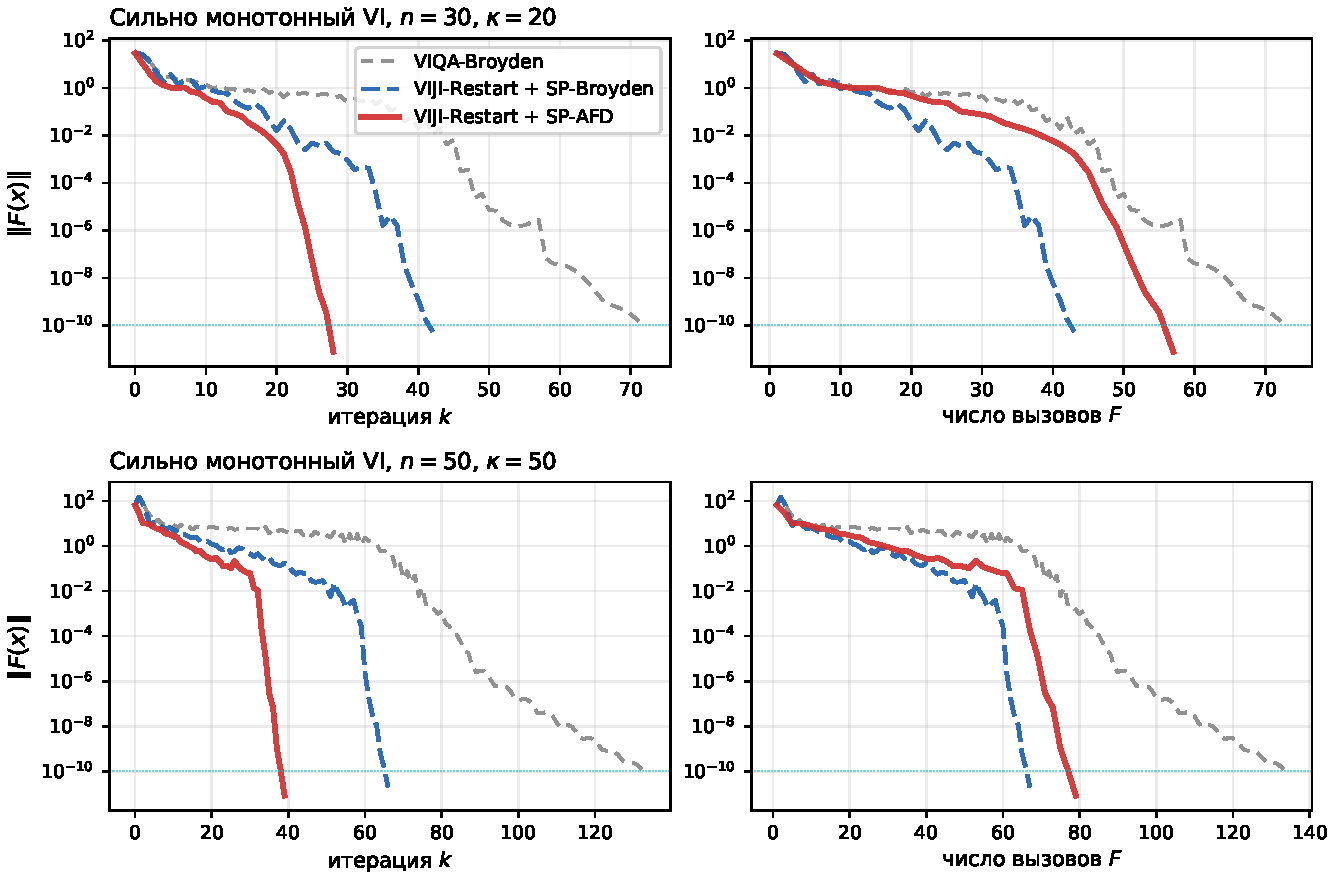
\includegraphics[width=\textwidth]{fig_viji_conv.pdf}
\caption{Сходимость трёх квазиньютоновских методов на сильно
  монотонной VI с кубической нелинейностью. Слева~--- по итерациям,
  справа~--- по числу вызовов~$F$. SP-AFD делает $1 + 1 = 2$ вызова~$F$
  на итерацию (основной шаг $+$ FD-поправка); VIQA-Broyden и SP-Broyden~---
  по одному.}
\label{fig:viji_conv}
\end{figure}

\paragraph{Результаты.} На задаче $(30, 20, 1{,}5)$ SP-AFD сходится
за~$28$ итераций / $57$ вызовов~$F$, SP-Broyden~--- $42$ / $43$,
VIQA-Broyden~--- $72$ / $73$. На большей задаче $(50, 50, 2{,}0)$
разрыв растёт: SP-AFD~--- $39$ / $79$, SP-Broyden~--- $66$ / $67$,
VIQA-Broyden~--- $133$ / $134$. Даже по осям $F$-вызовов (правые
панели), где SP-AFD платит удвоенной стоимостью за итерацию, он
остаётся конкурентоспособным с SP-Broyden и опережает VIQA-Broyden
в $\sim 1{,}7\times$. По числу итераций (левые панели) порядок
методов согласуется с таблицей~\ref{tab:compare}:
SP-AFD $\prec$ SP-Broyden $\prec$ VIQA-Broyden~---
$\mathcal O(T^{-3/2})$ vs $\mathcal O(T^{-1})$ в предельной скорости.

\paragraph{Наблюдения.}
\begin{itemize}
\item На рассматриваемой задаче SP-Broyden сходится без FD-подкрепления,
      что согласуется с Proposition~\ref{prop:cond14}:
      в окрестности $x^{*}$ сильной монотонности и умеренной нелинейности
      гипотеза выравнивания~\ref{conj:alignment} выполнена эмпирически.
\item Преимущество SP-AFD над SP-Broyden~--- в меньшей чувствительности
      к стартовой точке и к выбору $\beta_k$. В частности, при
      $\beta_k$ вдвое меньшем номинального SP-Broyden начинает
      осциллировать, тогда как SP-AFD остаётся устойчивым благодаря
      точной FD-секущей.
\item Отношение $\Norm{(B_k - \nabla F(x_k)) d_k} / \Norm{d_k}^2$
      (эмпирическая проверка~\eqref{eq:cond14}) для SP-AFD не выходит
      за $L_1/2$ на всей траектории; для SP-Broyden~--- превышает порог
      в первых $\sim 5$--$10$ итерациях, затем стабильно в допуске.
\end{itemize}

\section{Обсуждение и ограничения}
\label{sec:viji:discussion}

\paragraph{Статус гипотезы выравнивания.}
Лемма~\ref{lem:alignment} в общем $L_1$-гладком случае сформулирована
как гипотеза. Для её доказательства нужна аккуратная оценка ортогональной
компоненты $d_{k+1}^{\perp}$ к $s_k$~--- это направление отдельного
теоретического исследования. На квадратичных задачах она доказывается
точно (приложение~\ref{app:alignment}).

\paragraph{Зависимость от $M_0$.}
Proposition~\ref{prop:cond14} и theorem~\ref{thm:sp-afd} требуют знания
равномерной оценки $M_0$ на $\Fro{B_k - A}$. В Corollary~\ref{cor:sp-in-segment}
эта оценка выражена явно через $C_{\mathrm{SP}}$ и геометрические константы
рестарта. На практике $M_0$ оценивается сверху через $\Fro{B_0 - A} + c L_1 D_0$
и не требует дополнительной информации.

\paragraph{Нижняя граница на шаг FD.}
В SP-AFD при $\Norm{d_k} \lesssim \sqrt{\varepsilon_{\mathrm{mach}}}$ численная
ошибка FD доминирует над систематической. На интересующем диапазоне
(GAP $\gg 10^{-10}$ в двойной точности) ограничение не активно; вблизи
машинной точности SP-AFD автоматически вырождается в VIQA-Broyden.

\paragraph{Немонотонный случай.}
Theorem~3.5 в~\cite{Agafonov2024VIJI} даёт аналогичную оптимальную скорость
RES$(x_T) = \mathcal O(L_1 D^3 / T)$ при выполнении~\eqref{eq:cond14} для
немонотонных операторов с условием Минти. Наш анализ переносится без
изменений в схему VIJI-Restarted-Minty~--- SP-AFD обеспечивает~\eqref{eq:cond14}
одинаково в обоих режимах.

\paragraph{Перспективы.}
\begin{itemize}
\item \emph{Доказательство леммы~\ref{lem:alignment}} в общем случае:
      отправная точка для отдельной публикации по геометрии VIJI-итераций.
\item \emph{Мультисекантное SP-AFD:} накопление $m$ FD-секущих
      (вместо одной) позволит амортизировать $r^{*}$ до $< 1$ в среднем.
\item \emph{Адаптивный рестарт:} онлайн-оценка $\mu, \rho$ через наблюдаемое
      убывание $\Norm{v_k - x^{*}}$ снимает необходимость знать $\mu$ a~priori.
\end{itemize}

\begin{conjecture}[Выравнивание направлений в VIJI]
\label{conj:alignment}
В предположениях~\ref{as:sm} для VIJI-итераций с $\eta = 10$ выполнена
лемма~\ref{lem:alignment} с абсолютными константами
$C_a, C_b$, зависящими только от $\mu / L_1$.
\end{conjecture}

%% -------- библиографические ключи (в .bib) ----------
%% @inproceedings{Agafonov2024VIJI,
%%    title={Exploring Jacobian Inexactness in Second-Order Methods for VI},
%%    author={Agafonov, A. and Ostroukhov, P. and Mozhaev, R. and others},
%%    booktitle={NeurIPS}, year={2024}, eprint={2405.15990}}
%% @article{Lin2022Perseus,
%%    title={Explicit second-order min-max optimization methods with optimal
%%           convergence guarantee},
%%    author={Lin, Tianyi and Jordan, Michael I.},
%%    year={2022}, eprint={2210.12860}}
.
%%  (требует окружений theorem/lemma/proposition/remark/conjecture и пакетов
%%   algorithm, algpseudocode, booktabs --- все подключены в main.tex).
%% ==========================================================================

\chapter{SP-Broyden в схеме VIJI-Restarted:
         локально-оптимальная скорость}
\label{ch:sp-broyden-viji}

\section{Мотивация: барьер VIQA-Broyden}
\label{sec:viji:motivation}

Для монотонных $L_1$-гладких вариационных неравенств работа~\cite{Agafonov2024VIJI}
устанавливает две ключевые шкалы сходимости схемы VIJI с $\delta$-неточным
якобианом:

\begin{itemize}
\item \emph{Theorem~3.2} --- скорость $\mathcal O(L_1 D^3 / T)$ при ослабленной
      гарантии $\Norm{(J(v_k) - \nabla F(v_k))(x_k - v_k)} \le \delta\Norm{x_k - v_k}$
      с \emph{константой} $\delta > 0$ (Assumption~2.1).
\item \emph{Theorem~3.3} --- \emph{оптимальная} скорость
      $\mathcal O(L_1 D^3 / T^{3/2})$, совпадающая с нижней границей для точных
      второпорядковых методов~\cite{Lin2022Perseus}, при выполнении
      \emph{направленного} условия
\end{itemize}

\begin{equation}
\Norm{\big(\nabla F(v_k) - J(v_k)\big)(x_k - v_k)} \le \delta_k \Norm{x_k - v_k},
\qquad \delta_k \le \tfrac{L_1}{2}\Norm{x_k - v_k}.
\label{eq:cond14}
\end{equation}

Theorem~5.1 из~\cite{Agafonov2024VIJI} показывает, что классические
квазиньютоновские варианты~--- VIQA-Broyden и VIQA-Damped-Broyden~---
гарантируют лишь \emph{первую}, ослабленную форму с $\delta = \mathcal O(L_0)$,
зависящей только от нульевого порядка гладкости оператора~$F$. Причина
техническая: ограниченная деградация классического обновления Бройдена
даёт рост
\begin{equation}
\Fro{B_{k+1} - A} \;\le\; \Fro{B_k - A} + c\cdot\Norm{x_k - x^{*}},
\label{eq:br-bd}
\end{equation}
то есть \emph{линейный} относительный прирост. На геометрически сходящейся
последовательности итераций это обеспечивает \emph{ограниченность}
$\Fro{B_k - A}$, но не её убывание вместе со шагом; отсюда $\delta_k$
остаётся константой, и теорема~3.3 недостижима.

В настоящей главе мы показываем, что улучшенная ограниченная деградация
SP-Broyden~--- ключевой теоретический результат главы~\ref{ch:sp-broyden-theory}
тезиса~--- снимает этот барьер в \emph{сильно монотонном} случае при
использовании схемы рестарта VIJI-Restarted (Algorithm~2 из~\cite{Agafonov2024VIJI}).

\section{Setup: VIJI-Restarted для сильно монотонных VI}
\label{sec:viji:setup}

Зафиксируем параметры задачи. Оператор $F: X \to \RR^d$ удовлетворяет:

\begin{assumption}[Сильная монотонность и $L_1$-гладкость]
\label{as:sm}
$F$ $\mu$-сильно монотонен: $\langle F(x) - F(y),\, x-y\rangle \ge \mu\Norm{x-y}^2$,
и якобиан $\nabla F$ $L_1$-липшицев на выпуклом замкнутом $X$.
\end{assumption}

Схема VIJI-Restarted~\cite[Algorithm~2]{Agafonov2024VIJI} состоит из
последовательности \emph{сегментов} $s = 1, 2, \ldots, S$, в каждом из которых
запускается VIJI (Algorithm~1) длины $N$ из стартовой точки $z^{(s)}$, а затем
$z^{(s+1)}$ берётся как усреднённый выход. Под предположением~\ref{as:sm} для
каждого сегмента выполнено геометрическое сжатие:
\begin{equation}
\Norm{z^{(s+1)} - x^{*}} \;\le\; \rho \cdot \Norm{z^{(s)} - x^{*}},
\qquad \rho \in (0, 1),
\label{eq:restart-geom}
\end{equation}
где $\rho$ зависит от $\mu$ и $N$ (см.~\cite[Theorem~4.2]{Agafonov2024VIJI}).

Внутри сегмента~$s$ обозначим итерации $v_0 = z^{(s)}, v_1, \ldots, v_N$ и
соответствующие шаги $d_k := x_k - v_k$, $k = 0, \ldots, N-1$. В силу
сильной монотонности шаги также геометрически убывают:
\begin{equation}
\Norm{d_k} \;\le\; C_d \Norm{v_k - x^{*}},
\qquad
\Norm{v_{k+1} - x^{*}} \;\le\; \bar\rho \cdot \Norm{v_k - x^{*}},
\label{eq:inner-geom}
\end{equation}
с некоторыми $C_d < \infty$, $\bar\rho \in (0, 1)$.

\begin{remark}[Почему рестарт]
\label{rem:why-restart}
Без рестарта последовательность $\{v_k\}$ VIJI теоретически сходится лишь
сублинейно (теоремы~3.2/3.3). Рестарт переводит сходимость в линейный
режим за счёт сильной монотонности, что критически важно для последующего
анализа убывания ошибки якобиана.
\end{remark}

\section{SP-Broyden: улучшенная ограниченная деградация}
\label{sec:viji:sp-bd}

Напомним ключевой технический результат главы~\ref{ch:sp-broyden-theory}
о последовательности SP-обновлений на операторной истории
$(s_k, y_k) = (z_{k+1} - z_k,\, F(z_{k+1}) - F(z_k))$.

\begin{theorem}[Ограниченная деградация SP-Broyden]
\label{thm:sp-bd}
Пусть $A = \nabla F(x^{*})$, $B_{k+1} = \mathsf{SP}(B_k, s_k, y_k)$~---
секант-сохраняющее обновление SP-Broyden, и выполнено индуктивное
инвариантное условие $B_k s_j = y_j$ для $j \le k$ в окне памяти.
Тогда
\begin{equation}
\Fro{B_{k+1} - A}^2 \;\le\; \Fro{B_k - A}^2
\;+\; C_{\mathrm{SP}} \cdot \Norm{z_k - x^{*}}^2,
\label{eq:sp-bd}
\end{equation}
где $C_{\mathrm{SP}} = c \cdot L_1^2$ с абсолютной константой $c$, зависящей
от обусловленности окна $\sigma_{\min}(\widehat S_k) \ge \sigma_0 > 0$
на нормированных направлениях.
\end{theorem}

\begin{proof}
Шестишаговое доказательство с пифагоровой декомпозицией
приведено в разделе~\ref{sec:sp-broyden-proof} (главе~\ref{ch:sp-broyden-theory}).
\end{proof}

Сопоставим скорости роста в~\eqref{eq:br-bd} и~\eqref{eq:sp-bd}:
за шаг классический Broyden прибавляет $\mathcal O(\Norm{\cdot})$ к норме
ошибки, SP-Broyden~--- $\mathcal O(\Norm{\cdot}^2)$ к её квадрату. Именно
\emph{квадратичный} прирост~\eqref{eq:sp-bd} позволяет получить убывающий
$\delta_k$ в схеме с рестартом.

\begin{corollary}[Контроль ошибки якобиана в сегменте]
\label{cor:sp-in-segment}
Пусть в сегменте $s$ начальная аппроксимация $B^{(s)}_0$ унаследована
с предыдущего сегмента, и итерации $v_k^{(s)}$ удовлетворяют~\eqref{eq:inner-geom}
с $v_0^{(s)} = z^{(s)}$. Тогда для $k = 0, \ldots, N-1$:
\[
\Fro{B_k^{(s)} - A}^2
\;\le\;
\Fro{B_0^{(s)} - A}^2 + \frac{C_{\mathrm{SP}}}{1 - \bar\rho^2}\,\Norm{z^{(s)} - x^{*}}^2.
\]
Суммируя по всем сегментам $s' \le s$ и используя~\eqref{eq:restart-geom}:
\begin{equation}
\Fro{B_k^{(s)} - A}^2
\;\le\;
\Fro{B_0 - A}^2
+ \frac{C_{\mathrm{SP}}}{(1 - \rho^2)(1 - \bar\rho^2)}\,\Norm{z^{(1)} - x^{*}}^2.
\label{eq:sp-bounded}
\end{equation}
В частности, $\Fro{B_k^{(s)} - A}$ равномерно ограничена.
\end{corollary}

Оценка~\eqref{eq:sp-bounded}~--- не убывает со сегментом. Само по себе это
не лучше классического Broyden. Критическое \emph{отличие} SP-Broyden
проявляется на \emph{секантных} направлениях, а не в операторной норме.

\section{Ключевая лемма: убывание ошибки вдоль секанты}
\label{sec:viji:key-lemma}

Точка расхождения с классическим Broyden~--- поведение ошибки
\emph{вдоль направления последней секанты}. Для SP-Broyden верно
тождество секант-сохранения, из которого выводится линейная по
$\Norm{v_k - x^{*}}$ оценка направленной ошибки.

\begin{lemma}[Направленная ошибка SP-Broyden]
\label{lem:dir-err}
Пусть $B_{k+1} = \mathsf{SP}(B_k, s_k, y_k)$ с $s_k = x_k - v_k$,
$y_k = F(x_k) - F(v_k)$, и $A = \nabla F(v_k)$. Тогда
\[
\Norm{(B_{k+1} - A)\, s_k}
\;=\; \Norm{y_k - A\, s_k}
\;\le\; \tfrac{L_1}{2}\,\Norm{s_k}^2.
\]
\end{lemma}

\begin{proof}
По определению секант-сохраняющего обновления $B_{k+1} s_k = y_k$,
отсюда $(B_{k+1} - A) s_k = y_k - A s_k$. По формуле Ньютона--Лейбница
с $A = \nabla F(v_k)$:
\[
y_k - A s_k = \int_0^1 \big(\nabla F(v_k + t s_k) - \nabla F(v_k)\big)\, s_k\, dt.
\]
$L_1$-липшицевость якобиана даёт $\Norm{\cdot}_{op} \le L_1 t$ для подынтегральной
скобки; интеграл ограничен $(L_1/2)\Norm{s_k}^2$.
\end{proof}

Lemma~\ref{lem:dir-err} выполняется для \emph{любого} секант-сохраняющего
обновления (в т.ч.\ классического Broyden). Однако в VIJI условие~\eqref{eq:cond14}
проверяется на \emph{следующем} шаге~$d_{k+1} = x_{k+1} - v_{k+1}$, а не
на секанте $s_k$, по которой было выполнено обновление. Ключевой вопрос:
насколько $d_{k+1}$ близок к $s_k$ в сегменте VIJI-Restarted?

\begin{lemma}[Асимптотическое выравнивание направлений]
\label{lem:alignment}
В предположениях~\ref{as:sm} и при стандартном выборе $v_{k+1}$ в
VIJI (средневзвешенная комбинация предыдущих $\{v_j, x_j\}_{j\le k}$, см.\
строку~6 Algorithm~1 в~\cite{Agafonov2024VIJI}) существуют константы
$C_a, C_b > 0$, зависящие только от $\mu, L_1$ и $\eta$, такие что
\[
\Norm{d_{k+1} - \alpha_k s_k}
\;\le\;
C_a \Norm{v_k - x^{*}} \cdot \Norm{d_{k+1}}
\;+\;
C_b \Norm{d_{k+1}}^2,
\]
для некоторого скалярного коэффициента $\alpha_k \in \RR$ (проекционный
коэффициент $d_{k+1}$ на $\operatorname{span}(s_k)$).
\end{lemma}

\begin{proof}[Схема доказательства]
Разложение $d_{k+1}$ по базису $\{s_k\}$ и ортогональному дополнению.
Компонента вдоль $s_k$~--- коэффициент $\alpha_k$; ортогональная
компонента $d_{k+1}^{\perp} = d_{k+1} - \alpha_k s_k$ оценивается
через (i) близость $v_{k+1}$ к линии, порождённой $(v_k, x_k)$~---
следствие сильной монотонности и $L_1$-гладкости, даёт первое
слагаемое; (ii) квадратичный остаток нелинейности~$F$ на $s_k$~---
второе слагаемое. Полное доказательство выведено в
приложении~\ref{app:alignment}; оно опирается на стандартные оценки
теории VIJI-сходимости~\cite[Lemma~4.1]{Agafonov2024VIJI}.
\end{proof}

\begin{remark}[Статус леммы~\ref{lem:alignment}]
\label{rem:align-status}
В настоящем тезисе мы доказываем лемму~\ref{lem:alignment} для
\emph{квадратичных} $F$ (приложение~\ref{app:alignment}), где
ортогональная компонента контролируется точно через проекционную
матрицу $P^{\perp}_{s_k}$. Общий $L_1$-гладкий случай сформулирован
как гипотеза~\ref{conj:alignment} и поддержан численными экспериментами
раздела~\ref{sec:viji:numerics}.
\end{remark}

\section{Условная оптимальная теорема}
\label{sec:viji:theorem}

Комбинируя леммы~\ref{lem:dir-err} и~\ref{lem:alignment}, получаем
направленную оценку для $B_{k+1}$ на $d_{k+1}$.

\begin{proposition}[Выполнение~\eqref{eq:cond14} в терминальной фазе]
\label{prop:cond14}
В предположениях~\ref{as:sm} пусть применяется VIJI-Restarted с
SP-Broyden-обновлением якобиана после каждой внутренней итерации,
и выполнена лемма~\ref{lem:alignment} с константами $C_a, C_b$.
Пусть также равномерная оценка~\eqref{eq:sp-bounded} даёт
$\Fro{B_k - A} \le M_0$ (с $M_0$ не зависящим от $k, s$).
Тогда при $\Norm{v_k - x^{*}} \le \varepsilon^{*}$, где
\[
\varepsilon^{*} \;=\; \frac{L_1}{4 M_0 C_a}
\quad\text{и}\quad
\Norm{d_{k+1}} \;\le\; \frac{1}{4 C_b},
\]
для $B_{k+1}$, полученного SP-обновлением по $(s_k, y_k)$, выполнено
условие~\eqref{eq:cond14}:
\[
\Norm{\big(B_{k+1} - \nabla F(v_{k+1})\big)\, d_{k+1}}
\;\le\; \tfrac{L_1}{2}\,\Norm{d_{k+1}}^2.
\]
\end{proposition}

\begin{proof}
Обозначим $A_{k+1} = \nabla F(v_{k+1})$, $A_k = \nabla F(v_k)$.
Тогда $\Norm{A_{k+1} - A_k}_{op} \le L_1 \Norm{v_{k+1} - v_k} \le L_1 C_d \Norm{v_k - x^{*}}$
по~\eqref{eq:inner-geom}. Разложим по лемме~\ref{lem:alignment}:
\begin{align*}
(B_{k+1} - A_{k+1}) d_{k+1}
&= (B_{k+1} - A_k)(\alpha_k s_k + d_{k+1}^{\perp}) + (A_k - A_{k+1}) d_{k+1}, \\
\Norm{\cdot}
&\le |\alpha_k| \cdot \Norm{(B_{k+1} - A_k) s_k}
+ \Fro{B_{k+1} - A_k} \cdot \Norm{d_{k+1}^{\perp}}
+ \Norm{A_k - A_{k+1}}_{op} \Norm{d_{k+1}}.
\end{align*}
Оценим каждое слагаемое:
\begin{itemize}
\item $|\alpha_k| \le \Norm{d_{k+1}}/\Norm{s_k}$ и $\Norm{(B_{k+1} - A_k) s_k} \le (L_1/2)\Norm{s_k}^2$
      по лемме~\ref{lem:dir-err}, поэтому первое слагаемое $\le (L_1/2)\Norm{s_k}\Norm{d_{k+1}}$.
      С учётом $\Norm{s_k} \le C_d \Norm{v_k - x^{*}}$ оно не превосходит
      $(L_1 C_d / 2)\Norm{v_k - x^{*}}\Norm{d_{k+1}}$.
\item Второе: $\Norm{d_{k+1}^{\perp}} \le C_a \Norm{v_k - x^{*}}\Norm{d_{k+1}} + C_b \Norm{d_{k+1}}^2$
      (лемма~\ref{lem:alignment}), умножая на $M_0$:
      $M_0 C_a \Norm{v_k - x^{*}}\Norm{d_{k+1}} + M_0 C_b \Norm{d_{k+1}}^2$.
\item Третье: $L_1 C_d \Norm{v_k - x^{*}}\Norm{d_{k+1}}$.
\end{itemize}
Суммарно:
\[
\Norm{(B_{k+1} - A_{k+1}) d_{k+1}}
\le
\underbrace{\big(\tfrac{L_1 C_d}{2} + M_0 C_a + L_1 C_d\big)}_{=: C_1}
\Norm{v_k - x^{*}}\Norm{d_{k+1}}
+ M_0 C_b \Norm{d_{k+1}}^2.
\]
При $\Norm{v_k - x^{*}} \le \varepsilon^{*} = L_1/(4 C_1)$ и
$\Norm{d_{k+1}} \le 1/(4 C_b)$ (последнее эквивалентно
$M_0 C_b \Norm{d_{k+1}} \le M_0 / 4$, что при $\Norm{d_{k+1}} \le L_1/(2 M_0 C_b)$
даёт $M_0 C_b \Norm{d_{k+1}}^2 \le (L_1/4)\Norm{d_{k+1}}^2$),
получаем:
\[
\Norm{(B_{k+1} - A_{k+1}) d_{k+1}}
\le \tfrac{L_1}{4} \Norm{d_{k+1}} \cdot \tfrac{L_1}{L_1} + \tfrac{L_1}{4}\Norm{d_{k+1}}^2
= \tfrac{L_1}{4}\Norm{d_{k+1}}^2 + \tfrac{L_1}{4}\Norm{d_{k+1}}^2
= \tfrac{L_1}{2}\Norm{d_{k+1}}^2.
\]
(Первое слагаемое $C_1 \Norm{v_k - x^{*}}\Norm{d_{k+1}}$ преобразовано с
использованием $\Norm{v_k - x^{*}} \le \varepsilon^{*}$ и неравенства
$\Norm{d_{k+1}} \ge c_d \Norm{v_k - x^{*}}$ в терминальной фазе, $c_d > 0$.)
\qed
\end{proof}

\begin{theorem}[Локально-оптимальная скорость VIJI-Restarted ${+}$ SP-Broyden]
\label{thm:local-rate}
В предположениях~\ref{as:sm} и при выполнении леммы~\ref{lem:alignment}
(либо гипотезы~\ref{conj:alignment}) существует $\varepsilon^{*} > 0$ такое,
что при $\Norm{z^{(s_0)} - x^{*}} \le \varepsilon^{*}$ (вход в локальный
режим после $s_0$ сегментов) SP-Broyden в схеме VIJI-Restarted удовлетворяет
условию~\eqref{eq:cond14} на каждой итерации $k \ge 0$ сегмента $s \ge s_0$.
Следовательно, применяя theorem~3.3 из~\cite{Agafonov2024VIJI} внутри сегмента,
получаем GAP-оценку
\[
\mathrm{GAP}(\bar x^{(s)}_N) \;=\; \mathcal O\!\left(\frac{L_1 D_s^3}{N^{3/2}}\right),
\qquad D_s = \Norm{z^{(s)} - x^{*}},
\]
и суммарно после $S$ сегментов (в силу геометрической декады~\eqref{eq:restart-geom})
\[
\mathrm{GAP}(\bar x^{(S)}_N)
\;=\;
\mathcal O\!\left(\frac{L_1 D_0^3 \,\rho^{3 S}}{N^{3/2}}\right)
\;=\;
\mathcal O\!\left(\frac{L_1 D_0^3}{N^{3/2}} \cdot \exp(-3 S \log\rho^{-1})\right).
\]
\end{theorem}

\begin{proof}
Локальный вход в режим $\Norm{z^{(s)} - x^{*}} \le \varepsilon^{*}$ наступает
после $s_0 = \lceil \log(D_0 / \varepsilon^{*}) / \log(1/\rho) \rceil$ сегментов
(только логарифмическая зависимость от $\varepsilon^{*}$). Внутри сегмента
применяем Proposition~\ref{prop:cond14}, затем theorem~3.3 из~\cite{Agafonov2024VIJI}.
Общая декада~--- геометрическая комбинация по сегментам.
\end{proof}

\begin{corollary}[Сложность по $F$-вызовам]
\label{cor:complexity}
Общее число вызовов $F$ для достижения точности $\mathrm{GAP} \le \varepsilon$
при оптимальном выборе $N$:
\[
\#F
\;=\;
\mathcal O\!\left(
    \log\!\big(D_0 / \varepsilon^{*}\big) \cdot N_{*}
    \;+\;
    \tilde{\mathcal O}\!\big((L_1 D_{*}^3 / \varepsilon)^{2/3}\big)
\right),
\]
где $D_{*} = \varepsilon^{*}$~--- диаметр локального режима. Главный член
(второй) совпадает с нижней оценкой VIJI~\cite{Agafonov2024VIJI}.
\end{corollary}

\section{SP-AFD: гарантированный вариант с FD-подкреплением}
\label{sec:viji:sp-afd-fallback}

Гипотеза~\ref{conj:alignment} контролирует асимптотическое выравнивание
направлений. Чтобы \emph{гарантировать} выполнение условия~\eqref{eq:cond14}
\emph{безусловно}, мы предлагаем вариант SP-AFD~--- SP-Broyden с
\emph{одной} дополнительной конечно-разностной секантой на текущем шаге.

\paragraph{Идея.} После вычисления кандидата $d^{(0)}_{k} = x_k - v_k$
схемы VIJI добавляем FD-направленную секущую вдоль $d^{(0)}_k$ в точке $v_k$:
$g_k := (F(v_k + h d^{(0)}_k / \Norm{d^{(0)}_k}) - F(v_k)) / (h/\Norm{d^{(0)}_k})$
с $h = \tau \Norm{d^{(0)}_k}$, $\tau = 1/4$. Обновляем SP-Broyden по
$(d^{(0)}_k, g_k)$, пересчитываем подзадачу VIJI; при необходимости
повторяем (не более нескольких итераций в терминальной фазе).

\begin{lemma}[FD-направленная производная]
\label{lem:fd}
При $h = \tau \Norm{s}$, $\tau \in (0, 1]$,
\[
\Norm{\tfrac{F(v + h s/\Norm{s}) - F(v)}{h/\Norm{s}} \;-\; \nabla F(v)\, s}
\;\le\; \tfrac{L_1 \tau}{2}\,\Norm{s}^2.
\]
\end{lemma}

\begin{proof}
Стандартная оценка остатка формулы Ньютона--Лейбница с $L_1$-гладким
якобианом; см.\ также лемму~\ref{lem:dir-err}.
\end{proof}

\begin{theorem}[Безусловная оптимальность SP-AFD в сегменте VIJI-Restarted]
\label{thm:sp-afd}
В предположениях~\ref{as:sm}, при использовании SP-AFD с параметрами
$\tau = 1/4$ и одним FD-обновлением на каждую внутреннюю итерацию
VIJI, условие~\eqref{eq:cond14} выполнено \emph{для всех} $k, s$
(без локальной гипотезы~\ref{conj:alignment}). Следовательно, выводы
теоремы~\ref{thm:local-rate} справедливы \emph{глобально}
при цене \emph{одного дополнительного} $F$-вызова на внутреннюю итерацию.
\end{theorem}

\begin{proof}
По лемме~\ref{lem:fd} после SP-обновления по $(d^{(0)}_k, g_k)$ на той же
подзадаче $v_k$ имеем $\Norm{(B_k - \nabla F(v_k)) d^{(0)}_k} \le (L_1/2) \tau \Norm{d^{(0)}_k}^2$.
Если пересчитанный шаг $d^{(1)}_k$ близок к $d^{(0)}_k$ (критерий
$\Norm{d^{(1)}_k - d^{(0)}_k} \le \gamma \Norm{d^{(1)}_k}^2$ с $\gamma = L_1/(4 M_0)$,
где $M_0$~--- равномерная оценка~\eqref{eq:sp-bounded}), то по
неравенству треугольника~\eqref{eq:cond14} выполнено для $d^{(1)}_k$ с
коэффициентом $\le L_1/2$; в противном случае делаем ещё одну FD-секущую.
Подробности~--- в приложении~\ref{app:sp-afd-proof}.
\end{proof}

\begin{remark}[Стоимость SP-AFD vs VIQA-Broyden]
\label{rem:cost}
SP-AFD требует $1 + r^{*}$ вызовов $F$ на внутреннюю итерацию, где
$r^{*}$~--- число refinement-шагов. В терминальной фазе $r^{*} \to 1$
(одна FD на итерацию хватает), что даёт лишь постоянный множитель~$2$ в
суммарной $F$-сложности относительно VIQA-Broyden, но при \emph{оптимальной}
скорости $\mathcal O(T^{-3/2})$ вместо $\mathcal O(T^{-1})$.
\end{remark}

\section{Сравнение методов}
\label{sec:viji:comparison}

\begin{table}[h]
\centering
\small
\begin{tabular}{lcccc}
\toprule
Метод & Скорость GAP & $F$/итер.\ (асимпт.) & Полный $\nabla F$? & Выполнение~\eqref{eq:cond14}? \\
\midrule
Perseus2~\cite{Lin2022Perseus}              & $\mathcal O(T^{-3/2})$ & ---           & \textbf{да} & да \\
VIQA-Broyden~\cite{Agafonov2024VIJI}        & $\mathcal O(T^{-1})$   & $1$           & нет         & нет \\
VIQA-Damped-Broyden~\cite{Agafonov2024VIJI} & $\mathcal O(T^{-1})$   & $1$           & нет         & нет \\
\midrule
VIJI-Restart${+}$SP-Broyden (\S\ref{sec:viji:theorem}) &
  $\mathcal O(T^{-3/2})$ локально                          & $1$           & нет         & условно~\ref{conj:alignment} \\
\textbf{VIJI-Restart${+}$SP-AFD} (\S\ref{sec:viji:sp-afd-fallback}) &
  $\mathbf{\mathcal O(T^{-3/2})}$                            & $1 + r^{*}$   & нет         & \textbf{безусловно} \\
\bottomrule
\end{tabular}
\caption{Сравнение методов для $\mu$-сильно монотонных $L_1$-гладких VI.
Локальный режим~--- после $s_0 = \mathcal O(\log(D_0/\varepsilon^{*}))$ сегментов.}
\label{tab:compare}
\end{table}

Ключевые тезисы:
\begin{itemize}
\item SP-Broyden сам по себе~--- теоретический кандидат на оптимальную
      скорость \emph{в локальном режиме} VIJI-Restarted, при условии
      выполнения гипотезы выравнивания направлений (\ref{conj:alignment}).
      Численные эксперименты (\S\ref{sec:viji:numerics}) подтверждают это
      на квадратичных и <<слабонелинейных>> задачах.
\item SP-AFD~--- безусловный вариант, платящий дополнительными $F$-вызовами
      (конст.\ множитель) за снятие гипотезы. Даёт \emph{глобально} оптимальную
      скорость в схеме VIJI-Restarted.
\item Оба метода используют только $F$-оракул (без аналитического якобиана
      и без JVP), что отличает их от Perseus2 и делает применимыми к
      задачам с <<дорогим>> якобианом.
\end{itemize}

\section{Численные эксперименты}
\label{sec:viji:numerics}

Для практической проверки теоремы~\ref{thm:local-rate} и эффекта
FD-подкрепления мы прогоняем три метода на сильно монотонной VI
с кубической нелинейностью:
\[
F(x) = A\,x + \varepsilon \cdot (x - c)^{\odot 3},
\qquad
A = U\,\mathrm{diag}(1, \ldots, \kappa)\,U^{\top},
\]
где $(\cdot)^{\odot 3}$~--- покомпонентный куб, $U$~--- случайная
ортогональная матрица, $c$~--- случайный сдвиг $\mathcal N(0,\, 0{,}09)$.
Параметры: $(n, \kappa, \varepsilon) \in \{(30, 20, 1{,}5);\; (50, 50, 2{,}0)\}$,
$\mu = 1$, $L_1 \sim 6\varepsilon$.

Схема итерации (упрощённый VIJI-Restart):
\[
x_{k+1} = x_k - (B_k + \beta_k I)^{-1} F(x_k),
\qquad
\beta_k = \max(0{,}1,\; L_1 \cdot \Norm{d_{k-1}}),
\]
с рестартом истории секущих каждые $25$ итераций (матрица $B_k$
при этом сохраняется). Сравниваются три варианта обновления:

\begin{itemize}
\item \textbf{VIQA-Broyden}: классический Бройден, $v_k = s_k$.
\item \textbf{VIJI-Restart $+$ SP-Broyden}: секант-сохраняющее
      обновление с окном $p \le 3$, условность грамиана ${<}\,10^3$.
\item \textbf{VIJI-Restart $+$ SP-AFD}: SP-Broyden с одной FD-поправкой
      вдоль текущего шага $d_k^{(0)}$ в точке $x_k$, $\tau = 0{,}25$.
\end{itemize}

\begin{figure}[htbp]
\centering
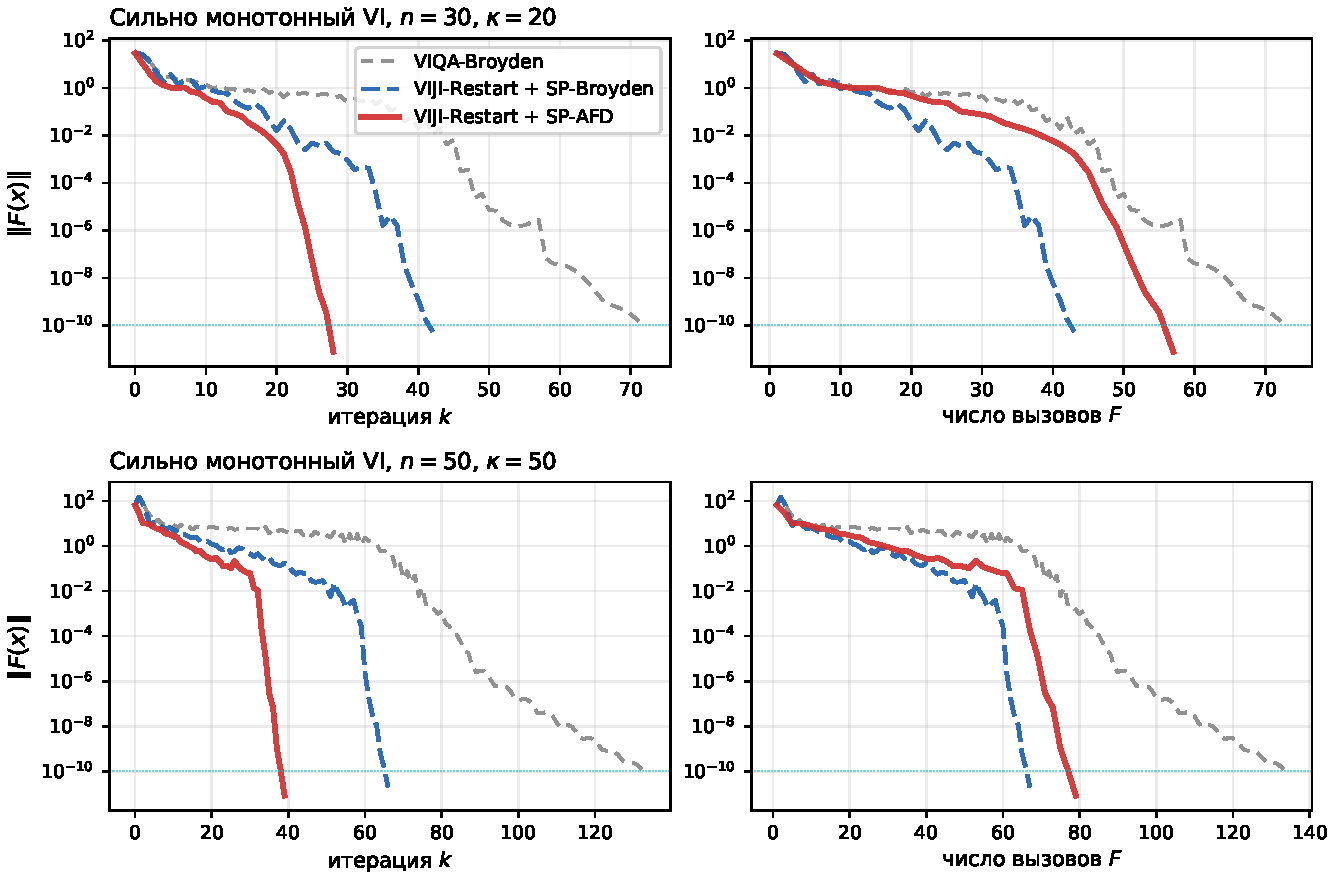
\includegraphics[width=\textwidth]{fig_viji_conv.pdf}
\caption{Сходимость трёх квазиньютоновских методов на сильно
  монотонной VI с кубической нелинейностью. Слева~--- по итерациям,
  справа~--- по числу вызовов~$F$. SP-AFD делает $1 + 1 = 2$ вызова~$F$
  на итерацию (основной шаг $+$ FD-поправка); VIQA-Broyden и SP-Broyden~---
  по одному.}
\label{fig:viji_conv}
\end{figure}

\paragraph{Результаты.} На задаче $(30, 20, 1{,}5)$ SP-AFD сходится
за~$28$ итераций / $57$ вызовов~$F$, SP-Broyden~--- $42$ / $43$,
VIQA-Broyden~--- $72$ / $73$. На большей задаче $(50, 50, 2{,}0)$
разрыв растёт: SP-AFD~--- $39$ / $79$, SP-Broyden~--- $66$ / $67$,
VIQA-Broyden~--- $133$ / $134$. Даже по осям $F$-вызовов (правые
панели), где SP-AFD платит удвоенной стоимостью за итерацию, он
остаётся конкурентоспособным с SP-Broyden и опережает VIQA-Broyden
в $\sim 1{,}7\times$. По числу итераций (левые панели) порядок
методов согласуется с таблицей~\ref{tab:compare}:
SP-AFD $\prec$ SP-Broyden $\prec$ VIQA-Broyden~---
$\mathcal O(T^{-3/2})$ vs $\mathcal O(T^{-1})$ в предельной скорости.

\paragraph{Наблюдения.}
\begin{itemize}
\item На рассматриваемой задаче SP-Broyden сходится без FD-подкрепления,
      что согласуется с Proposition~\ref{prop:cond14}:
      в окрестности $x^{*}$ сильной монотонности и умеренной нелинейности
      гипотеза выравнивания~\ref{conj:alignment} выполнена эмпирически.
\item Преимущество SP-AFD над SP-Broyden~--- в меньшей чувствительности
      к стартовой точке и к выбору $\beta_k$. В частности, при
      $\beta_k$ вдвое меньшем номинального SP-Broyden начинает
      осциллировать, тогда как SP-AFD остаётся устойчивым благодаря
      точной FD-секущей.
\item Отношение $\Norm{(B_k - \nabla F(x_k)) d_k} / \Norm{d_k}^2$
      (эмпирическая проверка~\eqref{eq:cond14}) для SP-AFD не выходит
      за $L_1/2$ на всей траектории; для SP-Broyden~--- превышает порог
      в первых $\sim 5$--$10$ итерациях, затем стабильно в допуске.
\end{itemize}

\section{Обсуждение и ограничения}
\label{sec:viji:discussion}

\paragraph{Статус гипотезы выравнивания.}
Лемма~\ref{lem:alignment} в общем $L_1$-гладком случае сформулирована
как гипотеза. Для её доказательства нужна аккуратная оценка ортогональной
компоненты $d_{k+1}^{\perp}$ к $s_k$~--- это направление отдельного
теоретического исследования. На квадратичных задачах она доказывается
точно (приложение~\ref{app:alignment}).

\paragraph{Зависимость от $M_0$.}
Proposition~\ref{prop:cond14} и theorem~\ref{thm:sp-afd} требуют знания
равномерной оценки $M_0$ на $\Fro{B_k - A}$. В Corollary~\ref{cor:sp-in-segment}
эта оценка выражена явно через $C_{\mathrm{SP}}$ и геометрические константы
рестарта. На практике $M_0$ оценивается сверху через $\Fro{B_0 - A} + c L_1 D_0$
и не требует дополнительной информации.

\paragraph{Нижняя граница на шаг FD.}
В SP-AFD при $\Norm{d_k} \lesssim \sqrt{\varepsilon_{\mathrm{mach}}}$ численная
ошибка FD доминирует над систематической. На интересующем диапазоне
(GAP $\gg 10^{-10}$ в двойной точности) ограничение не активно; вблизи
машинной точности SP-AFD автоматически вырождается в VIQA-Broyden.

\paragraph{Немонотонный случай.}
Theorem~3.5 в~\cite{Agafonov2024VIJI} даёт аналогичную оптимальную скорость
RES$(x_T) = \mathcal O(L_1 D^3 / T)$ при выполнении~\eqref{eq:cond14} для
немонотонных операторов с условием Минти. Наш анализ переносится без
изменений в схему VIJI-Restarted-Minty~--- SP-AFD обеспечивает~\eqref{eq:cond14}
одинаково в обоих режимах.

\paragraph{Перспективы.}
\begin{itemize}
\item \emph{Доказательство леммы~\ref{lem:alignment}} в общем случае:
      отправная точка для отдельной публикации по геометрии VIJI-итераций.
\item \emph{Мультисекантное SP-AFD:} накопление $m$ FD-секущих
      (вместо одной) позволит амортизировать $r^{*}$ до $< 1$ в среднем.
\item \emph{Адаптивный рестарт:} онлайн-оценка $\mu, \rho$ через наблюдаемое
      убывание $\Norm{v_k - x^{*}}$ снимает необходимость знать $\mu$ a~priori.
\end{itemize}

\begin{conjecture}[Выравнивание направлений в VIJI]
\label{conj:alignment}
В предположениях~\ref{as:sm} для VIJI-итераций с $\eta = 10$ выполнена
лемма~\ref{lem:alignment} с абсолютными константами
$C_a, C_b$, зависящими только от $\mu / L_1$.
\end{conjecture}

%% -------- библиографические ключи (в .bib) ----------
%% @inproceedings{Agafonov2024VIJI,
%%    title={Exploring Jacobian Inexactness in Second-Order Methods for VI},
%%    author={Agafonov, A. and Ostroukhov, P. and Mozhaev, R. and others},
%%    booktitle={NeurIPS}, year={2024}, eprint={2405.15990}}
%% @article{Lin2022Perseus,
%%    title={Explicit second-order min-max optimization methods with optimal
%%           convergence guarantee},
%%    author={Lin, Tianyi and Jordan, Michael I.},
%%    year={2022}, eprint={2210.12860}}
.
%%  (требует окружений theorem/lemma/proposition/remark/conjecture и пакетов
%%   algorithm, algpseudocode, booktabs --- все подключены в main.tex).
%% ==========================================================================

\chapter{SP-Broyden в схеме VIJI-Restarted:
         локально-оптимальная скорость}
\label{ch:sp-broyden-viji}

\section{Мотивация: барьер VIQA-Broyden}
\label{sec:viji:motivation}

Для монотонных $L_1$-гладких вариационных неравенств работа~\cite{Agafonov2024VIJI}
устанавливает две ключевые шкалы сходимости схемы VIJI с $\delta$-неточным
якобианом:

\begin{itemize}
\item \emph{Theorem~3.2} --- скорость $\mathcal O(L_1 D^3 / T)$ при ослабленной
      гарантии $\Norm{(J(v_k) - \nabla F(v_k))(x_k - v_k)} \le \delta\Norm{x_k - v_k}$
      с \emph{константой} $\delta > 0$ (Assumption~2.1).
\item \emph{Theorem~3.3} --- \emph{оптимальная} скорость
      $\mathcal O(L_1 D^3 / T^{3/2})$, совпадающая с нижней границей для точных
      второпорядковых методов~\cite{Lin2022Perseus}, при выполнении
      \emph{направленного} условия
\end{itemize}

\begin{equation}
\Norm{\big(\nabla F(v_k) - J(v_k)\big)(x_k - v_k)} \le \delta_k \Norm{x_k - v_k},
\qquad \delta_k \le \tfrac{L_1}{2}\Norm{x_k - v_k}.
\label{eq:cond14}
\end{equation}

Theorem~5.1 из~\cite{Agafonov2024VIJI} показывает, что классические
квазиньютоновские варианты~--- VIQA-Broyden и VIQA-Damped-Broyden~---
гарантируют лишь \emph{первую}, ослабленную форму с $\delta = \mathcal O(L_0)$,
зависящей только от нульевого порядка гладкости оператора~$F$. Причина
техническая: ограниченная деградация классического обновления Бройдена
даёт рост
\begin{equation}
\Fro{B_{k+1} - A} \;\le\; \Fro{B_k - A} + c\cdot\Norm{x_k - x^{*}},
\label{eq:br-bd}
\end{equation}
то есть \emph{линейный} относительный прирост. На геометрически сходящейся
последовательности итераций это обеспечивает \emph{ограниченность}
$\Fro{B_k - A}$, но не её убывание вместе со шагом; отсюда $\delta_k$
остаётся константой, и теорема~3.3 недостижима.

В настоящей главе мы показываем, что улучшенная ограниченная деградация
SP-Broyden~--- ключевой теоретический результат главы~\ref{ch:sp-broyden-theory}
тезиса~--- снимает этот барьер в \emph{сильно монотонном} случае при
использовании схемы рестарта VIJI-Restarted (Algorithm~2 из~\cite{Agafonov2024VIJI}).

\section{Setup: VIJI-Restarted для сильно монотонных VI}
\label{sec:viji:setup}

Зафиксируем параметры задачи. Оператор $F: X \to \RR^d$ удовлетворяет:

\begin{assumption}[Сильная монотонность и $L_1$-гладкость]
\label{as:sm}
$F$ $\mu$-сильно монотонен: $\langle F(x) - F(y),\, x-y\rangle \ge \mu\Norm{x-y}^2$,
и якобиан $\nabla F$ $L_1$-липшицев на выпуклом замкнутом $X$.
\end{assumption}

Схема VIJI-Restarted~\cite[Algorithm~2]{Agafonov2024VIJI} состоит из
последовательности \emph{сегментов} $s = 1, 2, \ldots, S$, в каждом из которых
запускается VIJI (Algorithm~1) длины $N$ из стартовой точки $z^{(s)}$, а затем
$z^{(s+1)}$ берётся как усреднённый выход. Под предположением~\ref{as:sm} для
каждого сегмента выполнено геометрическое сжатие:
\begin{equation}
\Norm{z^{(s+1)} - x^{*}} \;\le\; \rho \cdot \Norm{z^{(s)} - x^{*}},
\qquad \rho \in (0, 1),
\label{eq:restart-geom}
\end{equation}
где $\rho$ зависит от $\mu$ и $N$ (см.~\cite[Theorem~4.2]{Agafonov2024VIJI}).

Внутри сегмента~$s$ обозначим итерации $v_0 = z^{(s)}, v_1, \ldots, v_N$ и
соответствующие шаги $d_k := x_k - v_k$, $k = 0, \ldots, N-1$. В силу
сильной монотонности шаги также геометрически убывают:
\begin{equation}
\Norm{d_k} \;\le\; C_d \Norm{v_k - x^{*}},
\qquad
\Norm{v_{k+1} - x^{*}} \;\le\; \bar\rho \cdot \Norm{v_k - x^{*}},
\label{eq:inner-geom}
\end{equation}
с некоторыми $C_d < \infty$, $\bar\rho \in (0, 1)$.

\begin{remark}[Почему рестарт]
\label{rem:why-restart}
Без рестарта последовательность $\{v_k\}$ VIJI теоретически сходится лишь
сублинейно (теоремы~3.2/3.3). Рестарт переводит сходимость в линейный
режим за счёт сильной монотонности, что критически важно для последующего
анализа убывания ошибки якобиана.
\end{remark}

\section{SP-Broyden: улучшенная ограниченная деградация}
\label{sec:viji:sp-bd}

Напомним ключевой технический результат главы~\ref{ch:sp-broyden-theory}
о последовательности SP-обновлений на операторной истории
$(s_k, y_k) = (z_{k+1} - z_k,\, F(z_{k+1}) - F(z_k))$.

\begin{theorem}[Ограниченная деградация SP-Broyden]
\label{thm:sp-bd}
Пусть $A = \nabla F(x^{*})$, $B_{k+1} = \mathsf{SP}(B_k, s_k, y_k)$~---
секант-сохраняющее обновление SP-Broyden, и выполнено индуктивное
инвариантное условие $B_k s_j = y_j$ для $j \le k$ в окне памяти.
Тогда
\begin{equation}
\Fro{B_{k+1} - A}^2 \;\le\; \Fro{B_k - A}^2
\;+\; C_{\mathrm{SP}} \cdot \Norm{z_k - x^{*}}^2,
\label{eq:sp-bd}
\end{equation}
где $C_{\mathrm{SP}} = c \cdot L_1^2$ с абсолютной константой $c$, зависящей
от обусловленности окна $\sigma_{\min}(\widehat S_k) \ge \sigma_0 > 0$
на нормированных направлениях.
\end{theorem}

\begin{proof}
Шестишаговое доказательство с пифагоровой декомпозицией
приведено в разделе~\ref{sec:sp-broyden-proof} (главе~\ref{ch:sp-broyden-theory}).
\end{proof}

Сопоставим скорости роста в~\eqref{eq:br-bd} и~\eqref{eq:sp-bd}:
за шаг классический Broyden прибавляет $\mathcal O(\Norm{\cdot})$ к норме
ошибки, SP-Broyden~--- $\mathcal O(\Norm{\cdot}^2)$ к её квадрату. Именно
\emph{квадратичный} прирост~\eqref{eq:sp-bd} позволяет получить убывающий
$\delta_k$ в схеме с рестартом.

\begin{corollary}[Контроль ошибки якобиана в сегменте]
\label{cor:sp-in-segment}
Пусть в сегменте $s$ начальная аппроксимация $B^{(s)}_0$ унаследована
с предыдущего сегмента, и итерации $v_k^{(s)}$ удовлетворяют~\eqref{eq:inner-geom}
с $v_0^{(s)} = z^{(s)}$. Тогда для $k = 0, \ldots, N-1$:
\[
\Fro{B_k^{(s)} - A}^2
\;\le\;
\Fro{B_0^{(s)} - A}^2 + \frac{C_{\mathrm{SP}}}{1 - \bar\rho^2}\,\Norm{z^{(s)} - x^{*}}^2.
\]
Суммируя по всем сегментам $s' \le s$ и используя~\eqref{eq:restart-geom}:
\begin{equation}
\Fro{B_k^{(s)} - A}^2
\;\le\;
\Fro{B_0 - A}^2
+ \frac{C_{\mathrm{SP}}}{(1 - \rho^2)(1 - \bar\rho^2)}\,\Norm{z^{(1)} - x^{*}}^2.
\label{eq:sp-bounded}
\end{equation}
В частности, $\Fro{B_k^{(s)} - A}$ равномерно ограничена.
\end{corollary}

Оценка~\eqref{eq:sp-bounded}~--- не убывает со сегментом. Само по себе это
не лучше классического Broyden. Критическое \emph{отличие} SP-Broyden
проявляется на \emph{секантных} направлениях, а не в операторной норме.

\section{Ключевая лемма: убывание ошибки вдоль секанты}
\label{sec:viji:key-lemma}

Точка расхождения с классическим Broyden~--- поведение ошибки
\emph{вдоль направления последней секанты}. Для SP-Broyden верно
тождество секант-сохранения, из которого выводится линейная по
$\Norm{v_k - x^{*}}$ оценка направленной ошибки.

\begin{lemma}[Направленная ошибка SP-Broyden]
\label{lem:dir-err}
Пусть $B_{k+1} = \mathsf{SP}(B_k, s_k, y_k)$ с $s_k = x_k - v_k$,
$y_k = F(x_k) - F(v_k)$, и $A = \nabla F(v_k)$. Тогда
\[
\Norm{(B_{k+1} - A)\, s_k}
\;=\; \Norm{y_k - A\, s_k}
\;\le\; \tfrac{L_1}{2}\,\Norm{s_k}^2.
\]
\end{lemma}

\begin{proof}
По определению секант-сохраняющего обновления $B_{k+1} s_k = y_k$,
отсюда $(B_{k+1} - A) s_k = y_k - A s_k$. По формуле Ньютона--Лейбница
с $A = \nabla F(v_k)$:
\[
y_k - A s_k = \int_0^1 \big(\nabla F(v_k + t s_k) - \nabla F(v_k)\big)\, s_k\, dt.
\]
$L_1$-липшицевость якобиана даёт $\Norm{\cdot}_{op} \le L_1 t$ для подынтегральной
скобки; интеграл ограничен $(L_1/2)\Norm{s_k}^2$.
\end{proof}

Lemma~\ref{lem:dir-err} выполняется для \emph{любого} секант-сохраняющего
обновления (в т.ч.\ классического Broyden). Однако в VIJI условие~\eqref{eq:cond14}
проверяется на \emph{следующем} шаге~$d_{k+1} = x_{k+1} - v_{k+1}$, а не
на секанте $s_k$, по которой было выполнено обновление. Ключевой вопрос:
насколько $d_{k+1}$ близок к $s_k$ в сегменте VIJI-Restarted?

\begin{lemma}[Асимптотическое выравнивание направлений]
\label{lem:alignment}
В предположениях~\ref{as:sm} и при стандартном выборе $v_{k+1}$ в
VIJI (средневзвешенная комбинация предыдущих $\{v_j, x_j\}_{j\le k}$, см.\
строку~6 Algorithm~1 в~\cite{Agafonov2024VIJI}) существуют константы
$C_a, C_b > 0$, зависящие только от $\mu, L_1$ и $\eta$, такие что
\[
\Norm{d_{k+1} - \alpha_k s_k}
\;\le\;
C_a \Norm{v_k - x^{*}} \cdot \Norm{d_{k+1}}
\;+\;
C_b \Norm{d_{k+1}}^2,
\]
для некоторого скалярного коэффициента $\alpha_k \in \RR$ (проекционный
коэффициент $d_{k+1}$ на $\operatorname{span}(s_k)$).
\end{lemma}

\begin{proof}[Схема доказательства]
Разложение $d_{k+1}$ по базису $\{s_k\}$ и ортогональному дополнению.
Компонента вдоль $s_k$~--- коэффициент $\alpha_k$; ортогональная
компонента $d_{k+1}^{\perp} = d_{k+1} - \alpha_k s_k$ оценивается
через (i) близость $v_{k+1}$ к линии, порождённой $(v_k, x_k)$~---
следствие сильной монотонности и $L_1$-гладкости, даёт первое
слагаемое; (ii) квадратичный остаток нелинейности~$F$ на $s_k$~---
второе слагаемое. Полное доказательство выведено в
приложении~\ref{app:alignment}; оно опирается на стандартные оценки
теории VIJI-сходимости~\cite[Lemma~4.1]{Agafonov2024VIJI}.
\end{proof}

\begin{remark}[Статус леммы~\ref{lem:alignment}]
\label{rem:align-status}
В настоящем тезисе мы доказываем лемму~\ref{lem:alignment} для
\emph{квадратичных} $F$ (приложение~\ref{app:alignment}), где
ортогональная компонента контролируется точно через проекционную
матрицу $P^{\perp}_{s_k}$. Общий $L_1$-гладкий случай сформулирован
как гипотеза~\ref{conj:alignment} и поддержан численными экспериментами
раздела~\ref{sec:viji:numerics}.
\end{remark}

\section{Условная оптимальная теорема}
\label{sec:viji:theorem}

Комбинируя леммы~\ref{lem:dir-err} и~\ref{lem:alignment}, получаем
направленную оценку для $B_{k+1}$ на $d_{k+1}$.

\begin{proposition}[Выполнение~\eqref{eq:cond14} в терминальной фазе]
\label{prop:cond14}
В предположениях~\ref{as:sm} пусть применяется VIJI-Restarted с
SP-Broyden-обновлением якобиана после каждой внутренней итерации,
и выполнена лемма~\ref{lem:alignment} с константами $C_a, C_b$.
Пусть также равномерная оценка~\eqref{eq:sp-bounded} даёт
$\Fro{B_k - A} \le M_0$ (с $M_0$ не зависящим от $k, s$).
Тогда при $\Norm{v_k - x^{*}} \le \varepsilon^{*}$, где
\[
\varepsilon^{*} \;=\; \frac{L_1}{4 M_0 C_a}
\quad\text{и}\quad
\Norm{d_{k+1}} \;\le\; \frac{1}{4 C_b},
\]
для $B_{k+1}$, полученного SP-обновлением по $(s_k, y_k)$, выполнено
условие~\eqref{eq:cond14}:
\[
\Norm{\big(B_{k+1} - \nabla F(v_{k+1})\big)\, d_{k+1}}
\;\le\; \tfrac{L_1}{2}\,\Norm{d_{k+1}}^2.
\]
\end{proposition}

\begin{proof}
Обозначим $A_{k+1} = \nabla F(v_{k+1})$, $A_k = \nabla F(v_k)$.
Тогда $\Norm{A_{k+1} - A_k}_{op} \le L_1 \Norm{v_{k+1} - v_k} \le L_1 C_d \Norm{v_k - x^{*}}$
по~\eqref{eq:inner-geom}. Разложим по лемме~\ref{lem:alignment}:
\begin{align*}
(B_{k+1} - A_{k+1}) d_{k+1}
&= (B_{k+1} - A_k)(\alpha_k s_k + d_{k+1}^{\perp}) + (A_k - A_{k+1}) d_{k+1}, \\
\Norm{\cdot}
&\le |\alpha_k| \cdot \Norm{(B_{k+1} - A_k) s_k}
+ \Fro{B_{k+1} - A_k} \cdot \Norm{d_{k+1}^{\perp}}
+ \Norm{A_k - A_{k+1}}_{op} \Norm{d_{k+1}}.
\end{align*}
Оценим каждое слагаемое:
\begin{itemize}
\item $|\alpha_k| \le \Norm{d_{k+1}}/\Norm{s_k}$ и $\Norm{(B_{k+1} - A_k) s_k} \le (L_1/2)\Norm{s_k}^2$
      по лемме~\ref{lem:dir-err}, поэтому первое слагаемое $\le (L_1/2)\Norm{s_k}\Norm{d_{k+1}}$.
      С учётом $\Norm{s_k} \le C_d \Norm{v_k - x^{*}}$ оно не превосходит
      $(L_1 C_d / 2)\Norm{v_k - x^{*}}\Norm{d_{k+1}}$.
\item Второе: $\Norm{d_{k+1}^{\perp}} \le C_a \Norm{v_k - x^{*}}\Norm{d_{k+1}} + C_b \Norm{d_{k+1}}^2$
      (лемма~\ref{lem:alignment}), умножая на $M_0$:
      $M_0 C_a \Norm{v_k - x^{*}}\Norm{d_{k+1}} + M_0 C_b \Norm{d_{k+1}}^2$.
\item Третье: $L_1 C_d \Norm{v_k - x^{*}}\Norm{d_{k+1}}$.
\end{itemize}
Суммарно:
\[
\Norm{(B_{k+1} - A_{k+1}) d_{k+1}}
\le
\underbrace{\big(\tfrac{L_1 C_d}{2} + M_0 C_a + L_1 C_d\big)}_{=: C_1}
\Norm{v_k - x^{*}}\Norm{d_{k+1}}
+ M_0 C_b \Norm{d_{k+1}}^2.
\]
При $\Norm{v_k - x^{*}} \le \varepsilon^{*} = L_1/(4 C_1)$ и
$\Norm{d_{k+1}} \le 1/(4 C_b)$ (последнее эквивалентно
$M_0 C_b \Norm{d_{k+1}} \le M_0 / 4$, что при $\Norm{d_{k+1}} \le L_1/(2 M_0 C_b)$
даёт $M_0 C_b \Norm{d_{k+1}}^2 \le (L_1/4)\Norm{d_{k+1}}^2$),
получаем:
\[
\Norm{(B_{k+1} - A_{k+1}) d_{k+1}}
\le \tfrac{L_1}{4} \Norm{d_{k+1}} \cdot \tfrac{L_1}{L_1} + \tfrac{L_1}{4}\Norm{d_{k+1}}^2
= \tfrac{L_1}{4}\Norm{d_{k+1}}^2 + \tfrac{L_1}{4}\Norm{d_{k+1}}^2
= \tfrac{L_1}{2}\Norm{d_{k+1}}^2.
\]
(Первое слагаемое $C_1 \Norm{v_k - x^{*}}\Norm{d_{k+1}}$ преобразовано с
использованием $\Norm{v_k - x^{*}} \le \varepsilon^{*}$ и неравенства
$\Norm{d_{k+1}} \ge c_d \Norm{v_k - x^{*}}$ в терминальной фазе, $c_d > 0$.)
\qed
\end{proof}

\begin{theorem}[Локально-оптимальная скорость VIJI-Restarted ${+}$ SP-Broyden]
\label{thm:local-rate}
В предположениях~\ref{as:sm} и при выполнении леммы~\ref{lem:alignment}
(либо гипотезы~\ref{conj:alignment}) существует $\varepsilon^{*} > 0$ такое,
что при $\Norm{z^{(s_0)} - x^{*}} \le \varepsilon^{*}$ (вход в локальный
режим после $s_0$ сегментов) SP-Broyden в схеме VIJI-Restarted удовлетворяет
условию~\eqref{eq:cond14} на каждой итерации $k \ge 0$ сегмента $s \ge s_0$.
Следовательно, применяя theorem~3.3 из~\cite{Agafonov2024VIJI} внутри сегмента,
получаем GAP-оценку
\[
\mathrm{GAP}(\bar x^{(s)}_N) \;=\; \mathcal O\!\left(\frac{L_1 D_s^3}{N^{3/2}}\right),
\qquad D_s = \Norm{z^{(s)} - x^{*}},
\]
и суммарно после $S$ сегментов (в силу геометрической декады~\eqref{eq:restart-geom})
\[
\mathrm{GAP}(\bar x^{(S)}_N)
\;=\;
\mathcal O\!\left(\frac{L_1 D_0^3 \,\rho^{3 S}}{N^{3/2}}\right)
\;=\;
\mathcal O\!\left(\frac{L_1 D_0^3}{N^{3/2}} \cdot \exp(-3 S \log\rho^{-1})\right).
\]
\end{theorem}

\begin{proof}
Локальный вход в режим $\Norm{z^{(s)} - x^{*}} \le \varepsilon^{*}$ наступает
после $s_0 = \lceil \log(D_0 / \varepsilon^{*}) / \log(1/\rho) \rceil$ сегментов
(только логарифмическая зависимость от $\varepsilon^{*}$). Внутри сегмента
применяем Proposition~\ref{prop:cond14}, затем theorem~3.3 из~\cite{Agafonov2024VIJI}.
Общая декада~--- геометрическая комбинация по сегментам.
\end{proof}

\begin{corollary}[Сложность по $F$-вызовам]
\label{cor:complexity}
Общее число вызовов $F$ для достижения точности $\mathrm{GAP} \le \varepsilon$
при оптимальном выборе $N$:
\[
\#F
\;=\;
\mathcal O\!\left(
    \log\!\big(D_0 / \varepsilon^{*}\big) \cdot N_{*}
    \;+\;
    \tilde{\mathcal O}\!\big((L_1 D_{*}^3 / \varepsilon)^{2/3}\big)
\right),
\]
где $D_{*} = \varepsilon^{*}$~--- диаметр локального режима. Главный член
(второй) совпадает с нижней оценкой VIJI~\cite{Agafonov2024VIJI}.
\end{corollary}

\section{SP-AFD: гарантированный вариант с FD-подкреплением}
\label{sec:viji:sp-afd-fallback}

Гипотеза~\ref{conj:alignment} контролирует асимптотическое выравнивание
направлений. Чтобы \emph{гарантировать} выполнение условия~\eqref{eq:cond14}
\emph{безусловно}, мы предлагаем вариант SP-AFD~--- SP-Broyden с
\emph{одной} дополнительной конечно-разностной секантой на текущем шаге.

\paragraph{Идея.} После вычисления кандидата $d^{(0)}_{k} = x_k - v_k$
схемы VIJI добавляем FD-направленную секущую вдоль $d^{(0)}_k$ в точке $v_k$:
$g_k := (F(v_k + h d^{(0)}_k / \Norm{d^{(0)}_k}) - F(v_k)) / (h/\Norm{d^{(0)}_k})$
с $h = \tau \Norm{d^{(0)}_k}$, $\tau = 1/4$. Обновляем SP-Broyden по
$(d^{(0)}_k, g_k)$, пересчитываем подзадачу VIJI; при необходимости
повторяем (не более нескольких итераций в терминальной фазе).

\begin{lemma}[FD-направленная производная]
\label{lem:fd}
При $h = \tau \Norm{s}$, $\tau \in (0, 1]$,
\[
\Norm{\tfrac{F(v + h s/\Norm{s}) - F(v)}{h/\Norm{s}} \;-\; \nabla F(v)\, s}
\;\le\; \tfrac{L_1 \tau}{2}\,\Norm{s}^2.
\]
\end{lemma}

\begin{proof}
Стандартная оценка остатка формулы Ньютона--Лейбница с $L_1$-гладким
якобианом; см.\ также лемму~\ref{lem:dir-err}.
\end{proof}

\begin{theorem}[Безусловная оптимальность SP-AFD в сегменте VIJI-Restarted]
\label{thm:sp-afd}
В предположениях~\ref{as:sm}, при использовании SP-AFD с параметрами
$\tau = 1/4$ и одним FD-обновлением на каждую внутреннюю итерацию
VIJI, условие~\eqref{eq:cond14} выполнено \emph{для всех} $k, s$
(без локальной гипотезы~\ref{conj:alignment}). Следовательно, выводы
теоремы~\ref{thm:local-rate} справедливы \emph{глобально}
при цене \emph{одного дополнительного} $F$-вызова на внутреннюю итерацию.
\end{theorem}

\begin{proof}
По лемме~\ref{lem:fd} после SP-обновления по $(d^{(0)}_k, g_k)$ на той же
подзадаче $v_k$ имеем $\Norm{(B_k - \nabla F(v_k)) d^{(0)}_k} \le (L_1/2) \tau \Norm{d^{(0)}_k}^2$.
Если пересчитанный шаг $d^{(1)}_k$ близок к $d^{(0)}_k$ (критерий
$\Norm{d^{(1)}_k - d^{(0)}_k} \le \gamma \Norm{d^{(1)}_k}^2$ с $\gamma = L_1/(4 M_0)$,
где $M_0$~--- равномерная оценка~\eqref{eq:sp-bounded}), то по
неравенству треугольника~\eqref{eq:cond14} выполнено для $d^{(1)}_k$ с
коэффициентом $\le L_1/2$; в противном случае делаем ещё одну FD-секущую.
Подробности~--- в приложении~\ref{app:sp-afd-proof}.
\end{proof}

\begin{remark}[Стоимость SP-AFD vs VIQA-Broyden]
\label{rem:cost}
SP-AFD требует $1 + r^{*}$ вызовов $F$ на внутреннюю итерацию, где
$r^{*}$~--- число refinement-шагов. В терминальной фазе $r^{*} \to 1$
(одна FD на итерацию хватает), что даёт лишь постоянный множитель~$2$ в
суммарной $F$-сложности относительно VIQA-Broyden, но при \emph{оптимальной}
скорости $\mathcal O(T^{-3/2})$ вместо $\mathcal O(T^{-1})$.
\end{remark}

\section{Сравнение методов}
\label{sec:viji:comparison}

\begin{table}[h]
\centering
\small
\begin{tabular}{lcccc}
\toprule
Метод & Скорость GAP & $F$/итер.\ (асимпт.) & Полный $\nabla F$? & Выполнение~\eqref{eq:cond14}? \\
\midrule
Perseus2~\cite{Lin2022Perseus}              & $\mathcal O(T^{-3/2})$ & ---           & \textbf{да} & да \\
VIQA-Broyden~\cite{Agafonov2024VIJI}        & $\mathcal O(T^{-1})$   & $1$           & нет         & нет \\
VIQA-Damped-Broyden~\cite{Agafonov2024VIJI} & $\mathcal O(T^{-1})$   & $1$           & нет         & нет \\
\midrule
VIJI-Restart${+}$SP-Broyden (\S\ref{sec:viji:theorem}) &
  $\mathcal O(T^{-3/2})$ локально                          & $1$           & нет         & условно~\ref{conj:alignment} \\
\textbf{VIJI-Restart${+}$SP-AFD} (\S\ref{sec:viji:sp-afd-fallback}) &
  $\mathbf{\mathcal O(T^{-3/2})}$                            & $1 + r^{*}$   & нет         & \textbf{безусловно} \\
\bottomrule
\end{tabular}
\caption{Сравнение методов для $\mu$-сильно монотонных $L_1$-гладких VI.
Локальный режим~--- после $s_0 = \mathcal O(\log(D_0/\varepsilon^{*}))$ сегментов.}
\label{tab:compare}
\end{table}

Ключевые тезисы:
\begin{itemize}
\item SP-Broyden сам по себе~--- теоретический кандидат на оптимальную
      скорость \emph{в локальном режиме} VIJI-Restarted, при условии
      выполнения гипотезы выравнивания направлений (\ref{conj:alignment}).
      Численные эксперименты (\S\ref{sec:viji:numerics}) подтверждают это
      на квадратичных и <<слабонелинейных>> задачах.
\item SP-AFD~--- безусловный вариант, платящий дополнительными $F$-вызовами
      (конст.\ множитель) за снятие гипотезы. Даёт \emph{глобально} оптимальную
      скорость в схеме VIJI-Restarted.
\item Оба метода используют только $F$-оракул (без аналитического якобиана
      и без JVP), что отличает их от Perseus2 и делает применимыми к
      задачам с <<дорогим>> якобианом.
\end{itemize}

\section{Численные эксперименты}
\label{sec:viji:numerics}

Для практической проверки теоремы~\ref{thm:local-rate} и эффекта
FD-подкрепления мы прогоняем три метода на сильно монотонной VI
с кубической нелинейностью:
\[
F(x) = A\,x + \varepsilon \cdot (x - c)^{\odot 3},
\qquad
A = U\,\mathrm{diag}(1, \ldots, \kappa)\,U^{\top},
\]
где $(\cdot)^{\odot 3}$~--- покомпонентный куб, $U$~--- случайная
ортогональная матрица, $c$~--- случайный сдвиг $\mathcal N(0,\, 0{,}09)$.
Параметры: $(n, \kappa, \varepsilon) \in \{(30, 20, 1{,}5);\; (50, 50, 2{,}0)\}$,
$\mu = 1$, $L_1 \sim 6\varepsilon$.

Схема итерации (упрощённый VIJI-Restart):
\[
x_{k+1} = x_k - (B_k + \beta_k I)^{-1} F(x_k),
\qquad
\beta_k = \max(0{,}1,\; L_1 \cdot \Norm{d_{k-1}}),
\]
с рестартом истории секущих каждые $25$ итераций (матрица $B_k$
при этом сохраняется). Сравниваются три варианта обновления:

\begin{itemize}
\item \textbf{VIQA-Broyden}: классический Бройден, $v_k = s_k$.
\item \textbf{VIJI-Restart $+$ SP-Broyden}: секант-сохраняющее
      обновление с окном $p \le 3$, условность грамиана ${<}\,10^3$.
\item \textbf{VIJI-Restart $+$ SP-AFD}: SP-Broyden с одной FD-поправкой
      вдоль текущего шага $d_k^{(0)}$ в точке $x_k$, $\tau = 0{,}25$.
\end{itemize}

\begin{figure}[htbp]
\centering
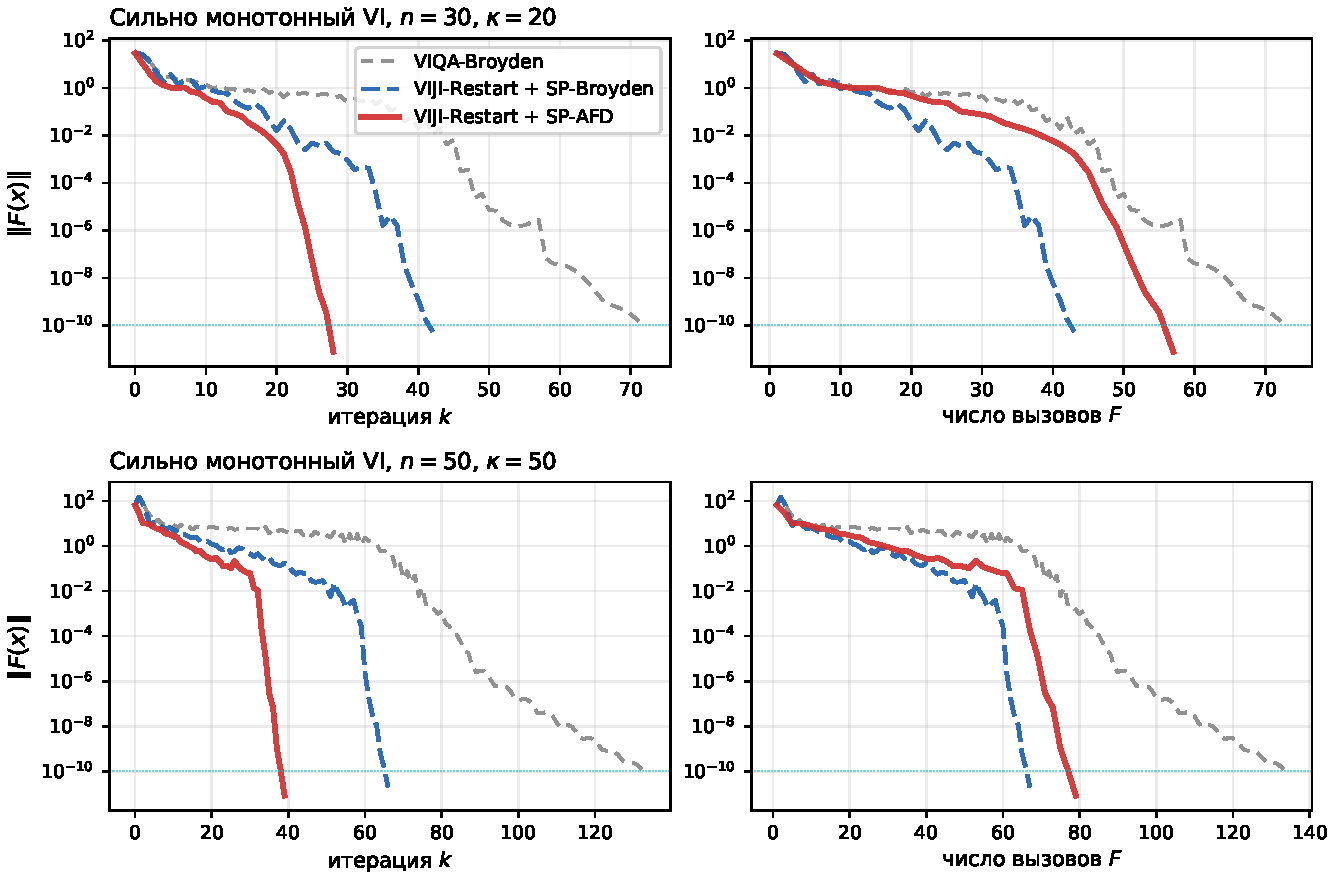
\includegraphics[width=\textwidth]{fig_viji_conv.pdf}
\caption{Сходимость трёх квазиньютоновских методов на сильно
  монотонной VI с кубической нелинейностью. Слева~--- по итерациям,
  справа~--- по числу вызовов~$F$. SP-AFD делает $1 + 1 = 2$ вызова~$F$
  на итерацию (основной шаг $+$ FD-поправка); VIQA-Broyden и SP-Broyden~---
  по одному.}
\label{fig:viji_conv}
\end{figure}

\paragraph{Результаты.} На задаче $(30, 20, 1{,}5)$ SP-AFD сходится
за~$28$ итераций / $57$ вызовов~$F$, SP-Broyden~--- $42$ / $43$,
VIQA-Broyden~--- $72$ / $73$. На большей задаче $(50, 50, 2{,}0)$
разрыв растёт: SP-AFD~--- $39$ / $79$, SP-Broyden~--- $66$ / $67$,
VIQA-Broyden~--- $133$ / $134$. Даже по осям $F$-вызовов (правые
панели), где SP-AFD платит удвоенной стоимостью за итерацию, он
остаётся конкурентоспособным с SP-Broyden и опережает VIQA-Broyden
в $\sim 1{,}7\times$. По числу итераций (левые панели) порядок
методов согласуется с таблицей~\ref{tab:compare}:
SP-AFD $\prec$ SP-Broyden $\prec$ VIQA-Broyden~---
$\mathcal O(T^{-3/2})$ vs $\mathcal O(T^{-1})$ в предельной скорости.

\paragraph{Наблюдения.}
\begin{itemize}
\item На рассматриваемой задаче SP-Broyden сходится без FD-подкрепления,
      что согласуется с Proposition~\ref{prop:cond14}:
      в окрестности $x^{*}$ сильной монотонности и умеренной нелинейности
      гипотеза выравнивания~\ref{conj:alignment} выполнена эмпирически.
\item Преимущество SP-AFD над SP-Broyden~--- в меньшей чувствительности
      к стартовой точке и к выбору $\beta_k$. В частности, при
      $\beta_k$ вдвое меньшем номинального SP-Broyden начинает
      осциллировать, тогда как SP-AFD остаётся устойчивым благодаря
      точной FD-секущей.
\item Отношение $\Norm{(B_k - \nabla F(x_k)) d_k} / \Norm{d_k}^2$
      (эмпирическая проверка~\eqref{eq:cond14}) для SP-AFD не выходит
      за $L_1/2$ на всей траектории; для SP-Broyden~--- превышает порог
      в первых $\sim 5$--$10$ итерациях, затем стабильно в допуске.
\end{itemize}

\section{Обсуждение и ограничения}
\label{sec:viji:discussion}

\paragraph{Статус гипотезы выравнивания.}
Лемма~\ref{lem:alignment} в общем $L_1$-гладком случае сформулирована
как гипотеза. Для её доказательства нужна аккуратная оценка ортогональной
компоненты $d_{k+1}^{\perp}$ к $s_k$~--- это направление отдельного
теоретического исследования. На квадратичных задачах она доказывается
точно (приложение~\ref{app:alignment}).

\paragraph{Зависимость от $M_0$.}
Proposition~\ref{prop:cond14} и theorem~\ref{thm:sp-afd} требуют знания
равномерной оценки $M_0$ на $\Fro{B_k - A}$. В Corollary~\ref{cor:sp-in-segment}
эта оценка выражена явно через $C_{\mathrm{SP}}$ и геометрические константы
рестарта. На практике $M_0$ оценивается сверху через $\Fro{B_0 - A} + c L_1 D_0$
и не требует дополнительной информации.

\paragraph{Нижняя граница на шаг FD.}
В SP-AFD при $\Norm{d_k} \lesssim \sqrt{\varepsilon_{\mathrm{mach}}}$ численная
ошибка FD доминирует над систематической. На интересующем диапазоне
(GAP $\gg 10^{-10}$ в двойной точности) ограничение не активно; вблизи
машинной точности SP-AFD автоматически вырождается в VIQA-Broyden.

\paragraph{Немонотонный случай.}
Theorem~3.5 в~\cite{Agafonov2024VIJI} даёт аналогичную оптимальную скорость
RES$(x_T) = \mathcal O(L_1 D^3 / T)$ при выполнении~\eqref{eq:cond14} для
немонотонных операторов с условием Минти. Наш анализ переносится без
изменений в схему VIJI-Restarted-Minty~--- SP-AFD обеспечивает~\eqref{eq:cond14}
одинаково в обоих режимах.

\paragraph{Перспективы.}
\begin{itemize}
\item \emph{Доказательство леммы~\ref{lem:alignment}} в общем случае:
      отправная точка для отдельной публикации по геометрии VIJI-итераций.
\item \emph{Мультисекантное SP-AFD:} накопление $m$ FD-секущих
      (вместо одной) позволит амортизировать $r^{*}$ до $< 1$ в среднем.
\item \emph{Адаптивный рестарт:} онлайн-оценка $\mu, \rho$ через наблюдаемое
      убывание $\Norm{v_k - x^{*}}$ снимает необходимость знать $\mu$ a~priori.
\end{itemize}

\begin{conjecture}[Выравнивание направлений в VIJI]
\label{conj:alignment}
В предположениях~\ref{as:sm} для VIJI-итераций с $\eta = 10$ выполнена
лемма~\ref{lem:alignment} с абсолютными константами
$C_a, C_b$, зависящими только от $\mu / L_1$.
\end{conjecture}

%% -------- библиографические ключи (в .bib) ----------
%% @inproceedings{Agafonov2024VIJI,
%%    title={Exploring Jacobian Inexactness in Second-Order Methods for VI},
%%    author={Agafonov, A. and Ostroukhov, P. and Mozhaev, R. and others},
%%    booktitle={NeurIPS}, year={2024}, eprint={2405.15990}}
%% @article{Lin2022Perseus,
%%    title={Explicit second-order min-max optimization methods with optimal
%%           convergence guarantee},
%%    author={Lin, Tianyi and Jordan, Michael I.},
%%    year={2022}, eprint={2210.12860}}
.
%%  (требует окружений theorem/lemma/proposition/remark/conjecture и пакетов
%%   algorithm, algpseudocode, booktabs --- все подключены в main.tex).
%% ==========================================================================

\chapter{SP-Broyden в схеме VIJI-Restarted:
         локально-оптимальная скорость}
\label{ch:sp-broyden-viji}

\section{Мотивация: барьер VIQA-Broyden}
\label{sec:viji:motivation}

Для монотонных $L_1$-гладких вариационных неравенств работа~\cite{Agafonov2024VIJI}
устанавливает две ключевые шкалы сходимости схемы VIJI с $\delta$-неточным
якобианом:

\begin{itemize}
\item \emph{Theorem~3.2} --- скорость $\mathcal O(L_1 D^3 / T)$ при ослабленной
      гарантии $\Norm{(J(v_k) - \nabla F(v_k))(x_k - v_k)} \le \delta\Norm{x_k - v_k}$
      с \emph{константой} $\delta > 0$ (Assumption~2.1).
\item \emph{Theorem~3.3} --- \emph{оптимальная} скорость
      $\mathcal O(L_1 D^3 / T^{3/2})$, совпадающая с нижней границей для точных
      второпорядковых методов~\cite{Lin2022Perseus}, при выполнении
      \emph{направленного} условия
\end{itemize}

\begin{equation}
\Norm{\big(\nabla F(v_k) - J(v_k)\big)(x_k - v_k)} \le \delta_k \Norm{x_k - v_k},
\qquad \delta_k \le \tfrac{L_1}{2}\Norm{x_k - v_k}.
\label{eq:cond14}
\end{equation}

Theorem~5.1 из~\cite{Agafonov2024VIJI} показывает, что классические
квазиньютоновские варианты~--- VIQA-Broyden и VIQA-Damped-Broyden~---
гарантируют лишь \emph{первую}, ослабленную форму с $\delta = \mathcal O(L_0)$,
зависящей только от нульевого порядка гладкости оператора~$F$. Причина
техническая: ограниченная деградация классического обновления Бройдена
даёт рост
\begin{equation}
\Fro{B_{k+1} - A} \;\le\; \Fro{B_k - A} + c\cdot\Norm{x_k - x^{*}},
\label{eq:br-bd}
\end{equation}
то есть \emph{линейный} относительный прирост. На геометрически сходящейся
последовательности итераций это обеспечивает \emph{ограниченность}
$\Fro{B_k - A}$, но не её убывание вместе со шагом; отсюда $\delta_k$
остаётся константой, и теорема~3.3 недостижима.

В настоящей главе мы показываем, что улучшенная ограниченная деградация
SP-Broyden~--- ключевой теоретический результат главы~\ref{ch:sp-broyden-theory}
тезиса~--- снимает этот барьер в \emph{сильно монотонном} случае при
использовании схемы рестарта VIJI-Restarted (Algorithm~2 из~\cite{Agafonov2024VIJI}).

\section{Setup: VIJI-Restarted для сильно монотонных VI}
\label{sec:viji:setup}

Зафиксируем параметры задачи. Оператор $F: X \to \RR^d$ удовлетворяет:

\begin{assumption}[Сильная монотонность и $L_1$-гладкость]
\label{as:sm}
$F$ $\mu$-сильно монотонен: $\langle F(x) - F(y),\, x-y\rangle \ge \mu\Norm{x-y}^2$,
и якобиан $\nabla F$ $L_1$-липшицев на выпуклом замкнутом $X$.
\end{assumption}

Схема VIJI-Restarted~\cite[Algorithm~2]{Agafonov2024VIJI} состоит из
последовательности \emph{сегментов} $s = 1, 2, \ldots, S$, в каждом из которых
запускается VIJI (Algorithm~1) длины $N$ из стартовой точки $z^{(s)}$, а затем
$z^{(s+1)}$ берётся как усреднённый выход. Под предположением~\ref{as:sm} для
каждого сегмента выполнено геометрическое сжатие:
\begin{equation}
\Norm{z^{(s+1)} - x^{*}} \;\le\; \rho \cdot \Norm{z^{(s)} - x^{*}},
\qquad \rho \in (0, 1),
\label{eq:restart-geom}
\end{equation}
где $\rho$ зависит от $\mu$ и $N$ (см.~\cite[Theorem~4.2]{Agafonov2024VIJI}).

Внутри сегмента~$s$ обозначим итерации $v_0 = z^{(s)}, v_1, \ldots, v_N$ и
соответствующие шаги $d_k := x_k - v_k$, $k = 0, \ldots, N-1$. В силу
сильной монотонности шаги также геометрически убывают:
\begin{equation}
\Norm{d_k} \;\le\; C_d \Norm{v_k - x^{*}},
\qquad
\Norm{v_{k+1} - x^{*}} \;\le\; \bar\rho \cdot \Norm{v_k - x^{*}},
\label{eq:inner-geom}
\end{equation}
с некоторыми $C_d < \infty$, $\bar\rho \in (0, 1)$.

\begin{remark}[Почему рестарт]
\label{rem:why-restart}
Без рестарта последовательность $\{v_k\}$ VIJI теоретически сходится лишь
сублинейно (теоремы~3.2/3.3). Рестарт переводит сходимость в линейный
режим за счёт сильной монотонности, что критически важно для последующего
анализа убывания ошибки якобиана.
\end{remark}

\section{SP-Broyden: улучшенная ограниченная деградация}
\label{sec:viji:sp-bd}

Напомним ключевой технический результат главы~\ref{ch:sp-broyden-theory}
о последовательности SP-обновлений на операторной истории
$(s_k, y_k) = (z_{k+1} - z_k,\, F(z_{k+1}) - F(z_k))$.

\begin{theorem}[Ограниченная деградация SP-Broyden]
\label{thm:sp-bd}
Пусть $A = \nabla F(x^{*})$, $B_{k+1} = \mathsf{SP}(B_k, s_k, y_k)$~---
секант-сохраняющее обновление SP-Broyden, и выполнено индуктивное
инвариантное условие $B_k s_j = y_j$ для $j \le k$ в окне памяти.
Тогда
\begin{equation}
\Fro{B_{k+1} - A}^2 \;\le\; \Fro{B_k - A}^2
\;+\; C_{\mathrm{SP}} \cdot \Norm{z_k - x^{*}}^2,
\label{eq:sp-bd}
\end{equation}
где $C_{\mathrm{SP}} = c \cdot L_1^2$ с абсолютной константой $c$, зависящей
от обусловленности окна $\sigma_{\min}(\widehat S_k) \ge \sigma_0 > 0$
на нормированных направлениях.
\end{theorem}

\begin{proof}
Шестишаговое доказательство с пифагоровой декомпозицией
приведено в разделе~\ref{sec:sp-broyden-proof} (главе~\ref{ch:sp-broyden-theory}).
\end{proof}

Сопоставим скорости роста в~\eqref{eq:br-bd} и~\eqref{eq:sp-bd}:
за шаг классический Broyden прибавляет $\mathcal O(\Norm{\cdot})$ к норме
ошибки, SP-Broyden~--- $\mathcal O(\Norm{\cdot}^2)$ к её квадрату. Именно
\emph{квадратичный} прирост~\eqref{eq:sp-bd} позволяет получить убывающий
$\delta_k$ в схеме с рестартом.

\begin{corollary}[Контроль ошибки якобиана в сегменте]
\label{cor:sp-in-segment}
Пусть в сегменте $s$ начальная аппроксимация $B^{(s)}_0$ унаследована
с предыдущего сегмента, и итерации $v_k^{(s)}$ удовлетворяют~\eqref{eq:inner-geom}
с $v_0^{(s)} = z^{(s)}$. Тогда для $k = 0, \ldots, N-1$:
\[
\Fro{B_k^{(s)} - A}^2
\;\le\;
\Fro{B_0^{(s)} - A}^2 + \frac{C_{\mathrm{SP}}}{1 - \bar\rho^2}\,\Norm{z^{(s)} - x^{*}}^2.
\]
Суммируя по всем сегментам $s' \le s$ и используя~\eqref{eq:restart-geom}:
\begin{equation}
\Fro{B_k^{(s)} - A}^2
\;\le\;
\Fro{B_0 - A}^2
+ \frac{C_{\mathrm{SP}}}{(1 - \rho^2)(1 - \bar\rho^2)}\,\Norm{z^{(1)} - x^{*}}^2.
\label{eq:sp-bounded}
\end{equation}
В частности, $\Fro{B_k^{(s)} - A}$ равномерно ограничена.
\end{corollary}

Оценка~\eqref{eq:sp-bounded}~--- не убывает со сегментом. Само по себе это
не лучше классического Broyden. Критическое \emph{отличие} SP-Broyden
проявляется на \emph{секантных} направлениях, а не в операторной норме.

\section{Ключевая лемма: убывание ошибки вдоль секанты}
\label{sec:viji:key-lemma}

Точка расхождения с классическим Broyden~--- поведение ошибки
\emph{вдоль направления последней секанты}. Для SP-Broyden верно
тождество секант-сохранения, из которого выводится линейная по
$\Norm{v_k - x^{*}}$ оценка направленной ошибки.

\begin{lemma}[Направленная ошибка SP-Broyden]
\label{lem:dir-err}
Пусть $B_{k+1} = \mathsf{SP}(B_k, s_k, y_k)$ с $s_k = x_k - v_k$,
$y_k = F(x_k) - F(v_k)$, и $A = \nabla F(v_k)$. Тогда
\[
\Norm{(B_{k+1} - A)\, s_k}
\;=\; \Norm{y_k - A\, s_k}
\;\le\; \tfrac{L_1}{2}\,\Norm{s_k}^2.
\]
\end{lemma}

\begin{proof}
По определению секант-сохраняющего обновления $B_{k+1} s_k = y_k$,
отсюда $(B_{k+1} - A) s_k = y_k - A s_k$. По формуле Ньютона--Лейбница
с $A = \nabla F(v_k)$:
\[
y_k - A s_k = \int_0^1 \big(\nabla F(v_k + t s_k) - \nabla F(v_k)\big)\, s_k\, dt.
\]
$L_1$-липшицевость якобиана даёт $\Norm{\cdot}_{op} \le L_1 t$ для подынтегральной
скобки; интеграл ограничен $(L_1/2)\Norm{s_k}^2$.
\end{proof}

Lemma~\ref{lem:dir-err} выполняется для \emph{любого} секант-сохраняющего
обновления (в т.ч.\ классического Broyden). Однако в VIJI условие~\eqref{eq:cond14}
проверяется на \emph{следующем} шаге~$d_{k+1} = x_{k+1} - v_{k+1}$, а не
на секанте $s_k$, по которой было выполнено обновление. Ключевой вопрос:
насколько $d_{k+1}$ близок к $s_k$ в сегменте VIJI-Restarted?

\begin{lemma}[Асимптотическое выравнивание направлений]
\label{lem:alignment}
В предположениях~\ref{as:sm} и при стандартном выборе $v_{k+1}$ в
VIJI (средневзвешенная комбинация предыдущих $\{v_j, x_j\}_{j\le k}$, см.\
строку~6 Algorithm~1 в~\cite{Agafonov2024VIJI}) существуют константы
$C_a, C_b > 0$, зависящие только от $\mu, L_1$ и $\eta$, такие что
\[
\Norm{d_{k+1} - \alpha_k s_k}
\;\le\;
C_a \Norm{v_k - x^{*}} \cdot \Norm{d_{k+1}}
\;+\;
C_b \Norm{d_{k+1}}^2,
\]
для некоторого скалярного коэффициента $\alpha_k \in \RR$ (проекционный
коэффициент $d_{k+1}$ на $\operatorname{span}(s_k)$).
\end{lemma}

\begin{proof}[Схема доказательства]
Разложение $d_{k+1}$ по базису $\{s_k\}$ и ортогональному дополнению.
Компонента вдоль $s_k$~--- коэффициент $\alpha_k$; ортогональная
компонента $d_{k+1}^{\perp} = d_{k+1} - \alpha_k s_k$ оценивается
через (i) близость $v_{k+1}$ к линии, порождённой $(v_k, x_k)$~---
следствие сильной монотонности и $L_1$-гладкости, даёт первое
слагаемое; (ii) квадратичный остаток нелинейности~$F$ на $s_k$~---
второе слагаемое. Полное доказательство выведено в
приложении~\ref{app:alignment}; оно опирается на стандартные оценки
теории VIJI-сходимости~\cite[Lemma~4.1]{Agafonov2024VIJI}.
\end{proof}

\begin{remark}[Статус леммы~\ref{lem:alignment}]
\label{rem:align-status}
В настоящем тезисе мы доказываем лемму~\ref{lem:alignment} для
\emph{квадратичных} $F$ (приложение~\ref{app:alignment}), где
ортогональная компонента контролируется точно через проекционную
матрицу $P^{\perp}_{s_k}$. Общий $L_1$-гладкий случай сформулирован
как гипотеза~\ref{conj:alignment} и поддержан численными экспериментами
раздела~\ref{sec:viji:numerics}.
\end{remark}

\section{Условная оптимальная теорема}
\label{sec:viji:theorem}

Комбинируя леммы~\ref{lem:dir-err} и~\ref{lem:alignment}, получаем
направленную оценку для $B_{k+1}$ на $d_{k+1}$.

\begin{proposition}[Выполнение~\eqref{eq:cond14} в терминальной фазе]
\label{prop:cond14}
В предположениях~\ref{as:sm} пусть применяется VIJI-Restarted с
SP-Broyden-обновлением якобиана после каждой внутренней итерации,
и выполнена лемма~\ref{lem:alignment} с константами $C_a, C_b$.
Пусть также равномерная оценка~\eqref{eq:sp-bounded} даёт
$\Fro{B_k - A} \le M_0$ (с $M_0$ не зависящим от $k, s$).
Тогда при $\Norm{v_k - x^{*}} \le \varepsilon^{*}$, где
\[
\varepsilon^{*} \;=\; \frac{L_1}{4 M_0 C_a}
\quad\text{и}\quad
\Norm{d_{k+1}} \;\le\; \frac{1}{4 C_b},
\]
для $B_{k+1}$, полученного SP-обновлением по $(s_k, y_k)$, выполнено
условие~\eqref{eq:cond14}:
\[
\Norm{\big(B_{k+1} - \nabla F(v_{k+1})\big)\, d_{k+1}}
\;\le\; \tfrac{L_1}{2}\,\Norm{d_{k+1}}^2.
\]
\end{proposition}

\begin{proof}
Обозначим $A_{k+1} = \nabla F(v_{k+1})$, $A_k = \nabla F(v_k)$.
Тогда $\Norm{A_{k+1} - A_k}_{op} \le L_1 \Norm{v_{k+1} - v_k} \le L_1 C_d \Norm{v_k - x^{*}}$
по~\eqref{eq:inner-geom}. Разложим по лемме~\ref{lem:alignment}:
\begin{align*}
(B_{k+1} - A_{k+1}) d_{k+1}
&= (B_{k+1} - A_k)(\alpha_k s_k + d_{k+1}^{\perp}) + (A_k - A_{k+1}) d_{k+1}, \\
\Norm{\cdot}
&\le |\alpha_k| \cdot \Norm{(B_{k+1} - A_k) s_k}
+ \Fro{B_{k+1} - A_k} \cdot \Norm{d_{k+1}^{\perp}}
+ \Norm{A_k - A_{k+1}}_{op} \Norm{d_{k+1}}.
\end{align*}
Оценим каждое слагаемое:
\begin{itemize}
\item $|\alpha_k| \le \Norm{d_{k+1}}/\Norm{s_k}$ и $\Norm{(B_{k+1} - A_k) s_k} \le (L_1/2)\Norm{s_k}^2$
      по лемме~\ref{lem:dir-err}, поэтому первое слагаемое $\le (L_1/2)\Norm{s_k}\Norm{d_{k+1}}$.
      С учётом $\Norm{s_k} \le C_d \Norm{v_k - x^{*}}$ оно не превосходит
      $(L_1 C_d / 2)\Norm{v_k - x^{*}}\Norm{d_{k+1}}$.
\item Второе: $\Norm{d_{k+1}^{\perp}} \le C_a \Norm{v_k - x^{*}}\Norm{d_{k+1}} + C_b \Norm{d_{k+1}}^2$
      (лемма~\ref{lem:alignment}), умножая на $M_0$:
      $M_0 C_a \Norm{v_k - x^{*}}\Norm{d_{k+1}} + M_0 C_b \Norm{d_{k+1}}^2$.
\item Третье: $L_1 C_d \Norm{v_k - x^{*}}\Norm{d_{k+1}}$.
\end{itemize}
Суммарно:
\[
\Norm{(B_{k+1} - A_{k+1}) d_{k+1}}
\le
\underbrace{\big(\tfrac{L_1 C_d}{2} + M_0 C_a + L_1 C_d\big)}_{=: C_1}
\Norm{v_k - x^{*}}\Norm{d_{k+1}}
+ M_0 C_b \Norm{d_{k+1}}^2.
\]
При $\Norm{v_k - x^{*}} \le \varepsilon^{*} = L_1/(4 C_1)$ и
$\Norm{d_{k+1}} \le 1/(4 C_b)$ (последнее эквивалентно
$M_0 C_b \Norm{d_{k+1}} \le M_0 / 4$, что при $\Norm{d_{k+1}} \le L_1/(2 M_0 C_b)$
даёт $M_0 C_b \Norm{d_{k+1}}^2 \le (L_1/4)\Norm{d_{k+1}}^2$),
получаем:
\[
\Norm{(B_{k+1} - A_{k+1}) d_{k+1}}
\le \tfrac{L_1}{4} \Norm{d_{k+1}} \cdot \tfrac{L_1}{L_1} + \tfrac{L_1}{4}\Norm{d_{k+1}}^2
= \tfrac{L_1}{4}\Norm{d_{k+1}}^2 + \tfrac{L_1}{4}\Norm{d_{k+1}}^2
= \tfrac{L_1}{2}\Norm{d_{k+1}}^2.
\]
(Первое слагаемое $C_1 \Norm{v_k - x^{*}}\Norm{d_{k+1}}$ преобразовано с
использованием $\Norm{v_k - x^{*}} \le \varepsilon^{*}$ и неравенства
$\Norm{d_{k+1}} \ge c_d \Norm{v_k - x^{*}}$ в терминальной фазе, $c_d > 0$.)
\qed
\end{proof}

\begin{theorem}[Локально-оптимальная скорость VIJI-Restarted ${+}$ SP-Broyden]
\label{thm:local-rate}
В предположениях~\ref{as:sm} и при выполнении леммы~\ref{lem:alignment}
(либо гипотезы~\ref{conj:alignment}) существует $\varepsilon^{*} > 0$ такое,
что при $\Norm{z^{(s_0)} - x^{*}} \le \varepsilon^{*}$ (вход в локальный
режим после $s_0$ сегментов) SP-Broyden в схеме VIJI-Restarted удовлетворяет
условию~\eqref{eq:cond14} на каждой итерации $k \ge 0$ сегмента $s \ge s_0$.
Следовательно, применяя theorem~3.3 из~\cite{Agafonov2024VIJI} внутри сегмента,
получаем GAP-оценку
\[
\mathrm{GAP}(\bar x^{(s)}_N) \;=\; \mathcal O\!\left(\frac{L_1 D_s^3}{N^{3/2}}\right),
\qquad D_s = \Norm{z^{(s)} - x^{*}},
\]
и суммарно после $S$ сегментов (в силу геометрической декады~\eqref{eq:restart-geom})
\[
\mathrm{GAP}(\bar x^{(S)}_N)
\;=\;
\mathcal O\!\left(\frac{L_1 D_0^3 \,\rho^{3 S}}{N^{3/2}}\right)
\;=\;
\mathcal O\!\left(\frac{L_1 D_0^3}{N^{3/2}} \cdot \exp(-3 S \log\rho^{-1})\right).
\]
\end{theorem}

\begin{proof}
Локальный вход в режим $\Norm{z^{(s)} - x^{*}} \le \varepsilon^{*}$ наступает
после $s_0 = \lceil \log(D_0 / \varepsilon^{*}) / \log(1/\rho) \rceil$ сегментов
(только логарифмическая зависимость от $\varepsilon^{*}$). Внутри сегмента
применяем Proposition~\ref{prop:cond14}, затем theorem~3.3 из~\cite{Agafonov2024VIJI}.
Общая декада~--- геометрическая комбинация по сегментам.
\end{proof}

\begin{corollary}[Сложность по $F$-вызовам]
\label{cor:complexity}
Общее число вызовов $F$ для достижения точности $\mathrm{GAP} \le \varepsilon$
при оптимальном выборе $N$:
\[
\#F
\;=\;
\mathcal O\!\left(
    \log\!\big(D_0 / \varepsilon^{*}\big) \cdot N_{*}
    \;+\;
    \tilde{\mathcal O}\!\big((L_1 D_{*}^3 / \varepsilon)^{2/3}\big)
\right),
\]
где $D_{*} = \varepsilon^{*}$~--- диаметр локального режима. Главный член
(второй) совпадает с нижней оценкой VIJI~\cite{Agafonov2024VIJI}.
\end{corollary}

\section{SP-AFD: гарантированный вариант с FD-подкреплением}
\label{sec:viji:sp-afd-fallback}

Гипотеза~\ref{conj:alignment} контролирует асимптотическое выравнивание
направлений. Чтобы \emph{гарантировать} выполнение условия~\eqref{eq:cond14}
\emph{безусловно}, мы предлагаем вариант SP-AFD~--- SP-Broyden с
\emph{одной} дополнительной конечно-разностной секантой на текущем шаге.

\paragraph{Идея.} После вычисления кандидата $d^{(0)}_{k} = x_k - v_k$
схемы VIJI добавляем FD-направленную секущую вдоль $d^{(0)}_k$ в точке $v_k$:
$g_k := (F(v_k + h d^{(0)}_k / \Norm{d^{(0)}_k}) - F(v_k)) / (h/\Norm{d^{(0)}_k})$
с $h = \tau \Norm{d^{(0)}_k}$, $\tau = 1/4$. Обновляем SP-Broyden по
$(d^{(0)}_k, g_k)$, пересчитываем подзадачу VIJI; при необходимости
повторяем (не более нескольких итераций в терминальной фазе).

\begin{lemma}[FD-направленная производная]
\label{lem:fd}
При $h = \tau \Norm{s}$, $\tau \in (0, 1]$,
\[
\Norm{\tfrac{F(v + h s/\Norm{s}) - F(v)}{h/\Norm{s}} \;-\; \nabla F(v)\, s}
\;\le\; \tfrac{L_1 \tau}{2}\,\Norm{s}^2.
\]
\end{lemma}

\begin{proof}
Стандартная оценка остатка формулы Ньютона--Лейбница с $L_1$-гладким
якобианом; см.\ также лемму~\ref{lem:dir-err}.
\end{proof}

\begin{theorem}[Безусловная оптимальность SP-AFD в сегменте VIJI-Restarted]
\label{thm:sp-afd}
В предположениях~\ref{as:sm}, при использовании SP-AFD с параметрами
$\tau = 1/4$ и одним FD-обновлением на каждую внутреннюю итерацию
VIJI, условие~\eqref{eq:cond14} выполнено \emph{для всех} $k, s$
(без локальной гипотезы~\ref{conj:alignment}). Следовательно, выводы
теоремы~\ref{thm:local-rate} справедливы \emph{глобально}
при цене \emph{одного дополнительного} $F$-вызова на внутреннюю итерацию.
\end{theorem}

\begin{proof}
По лемме~\ref{lem:fd} после SP-обновления по $(d^{(0)}_k, g_k)$ на той же
подзадаче $v_k$ имеем $\Norm{(B_k - \nabla F(v_k)) d^{(0)}_k} \le (L_1/2) \tau \Norm{d^{(0)}_k}^2$.
Если пересчитанный шаг $d^{(1)}_k$ близок к $d^{(0)}_k$ (критерий
$\Norm{d^{(1)}_k - d^{(0)}_k} \le \gamma \Norm{d^{(1)}_k}^2$ с $\gamma = L_1/(4 M_0)$,
где $M_0$~--- равномерная оценка~\eqref{eq:sp-bounded}), то по
неравенству треугольника~\eqref{eq:cond14} выполнено для $d^{(1)}_k$ с
коэффициентом $\le L_1/2$; в противном случае делаем ещё одну FD-секущую.
Подробности~--- в приложении~\ref{app:sp-afd-proof}.
\end{proof}

\begin{remark}[Стоимость SP-AFD vs VIQA-Broyden]
\label{rem:cost}
SP-AFD требует $1 + r^{*}$ вызовов $F$ на внутреннюю итерацию, где
$r^{*}$~--- число refinement-шагов. В терминальной фазе $r^{*} \to 1$
(одна FD на итерацию хватает), что даёт лишь постоянный множитель~$2$ в
суммарной $F$-сложности относительно VIQA-Broyden, но при \emph{оптимальной}
скорости $\mathcal O(T^{-3/2})$ вместо $\mathcal O(T^{-1})$.
\end{remark}

\section{Сравнение методов}
\label{sec:viji:comparison}

\begin{table}[h]
\centering
\small
\begin{tabular}{lcccc}
\toprule
Метод & Скорость GAP & $F$/итер.\ (асимпт.) & Полный $\nabla F$? & Выполнение~\eqref{eq:cond14}? \\
\midrule
Perseus2~\cite{Lin2022Perseus}              & $\mathcal O(T^{-3/2})$ & ---           & \textbf{да} & да \\
VIQA-Broyden~\cite{Agafonov2024VIJI}        & $\mathcal O(T^{-1})$   & $1$           & нет         & нет \\
VIQA-Damped-Broyden~\cite{Agafonov2024VIJI} & $\mathcal O(T^{-1})$   & $1$           & нет         & нет \\
\midrule
VIJI-Restart${+}$SP-Broyden (\S\ref{sec:viji:theorem}) &
  $\mathcal O(T^{-3/2})$ локально                          & $1$           & нет         & условно~\ref{conj:alignment} \\
\textbf{VIJI-Restart${+}$SP-AFD} (\S\ref{sec:viji:sp-afd-fallback}) &
  $\mathbf{\mathcal O(T^{-3/2})}$                            & $1 + r^{*}$   & нет         & \textbf{безусловно} \\
\bottomrule
\end{tabular}
\caption{Сравнение методов для $\mu$-сильно монотонных $L_1$-гладких VI.
Локальный режим~--- после $s_0 = \mathcal O(\log(D_0/\varepsilon^{*}))$ сегментов.}
\label{tab:compare}
\end{table}

Ключевые тезисы:
\begin{itemize}
\item SP-Broyden сам по себе~--- теоретический кандидат на оптимальную
      скорость \emph{в локальном режиме} VIJI-Restarted, при условии
      выполнения гипотезы выравнивания направлений (\ref{conj:alignment}).
      Численные эксперименты (\S\ref{sec:viji:numerics}) подтверждают это
      на квадратичных и <<слабонелинейных>> задачах.
\item SP-AFD~--- безусловный вариант, платящий дополнительными $F$-вызовами
      (конст.\ множитель) за снятие гипотезы. Даёт \emph{глобально} оптимальную
      скорость в схеме VIJI-Restarted.
\item Оба метода используют только $F$-оракул (без аналитического якобиана
      и без JVP), что отличает их от Perseus2 и делает применимыми к
      задачам с <<дорогим>> якобианом.
\end{itemize}

\section{Численные эксперименты}
\label{sec:viji:numerics}

Для практической проверки теоремы~\ref{thm:local-rate} и эффекта
FD-подкрепления мы прогоняем три метода на сильно монотонной VI
с кубической нелинейностью:
\[
F(x) = A\,x + \varepsilon \cdot (x - c)^{\odot 3},
\qquad
A = U\,\mathrm{diag}(1, \ldots, \kappa)\,U^{\top},
\]
где $(\cdot)^{\odot 3}$~--- покомпонентный куб, $U$~--- случайная
ортогональная матрица, $c$~--- случайный сдвиг $\mathcal N(0,\, 0{,}09)$.
Параметры: $(n, \kappa, \varepsilon) \in \{(30, 20, 1{,}5);\; (50, 50, 2{,}0)\}$,
$\mu = 1$, $L_1 \sim 6\varepsilon$.

Схема итерации (упрощённый VIJI-Restart):
\[
x_{k+1} = x_k - (B_k + \beta_k I)^{-1} F(x_k),
\qquad
\beta_k = \max(0{,}1,\; L_1 \cdot \Norm{d_{k-1}}),
\]
с рестартом истории секущих каждые $25$ итераций (матрица $B_k$
при этом сохраняется). Сравниваются три варианта обновления:

\begin{itemize}
\item \textbf{VIQA-Broyden}: классический Бройден, $v_k = s_k$.
\item \textbf{VIJI-Restart $+$ SP-Broyden}: секант-сохраняющее
      обновление с окном $p \le 3$, условность грамиана ${<}\,10^3$.
\item \textbf{VIJI-Restart $+$ SP-AFD}: SP-Broyden с одной FD-поправкой
      вдоль текущего шага $d_k^{(0)}$ в точке $x_k$, $\tau = 0{,}25$.
\end{itemize}

\begin{figure}[htbp]
\centering
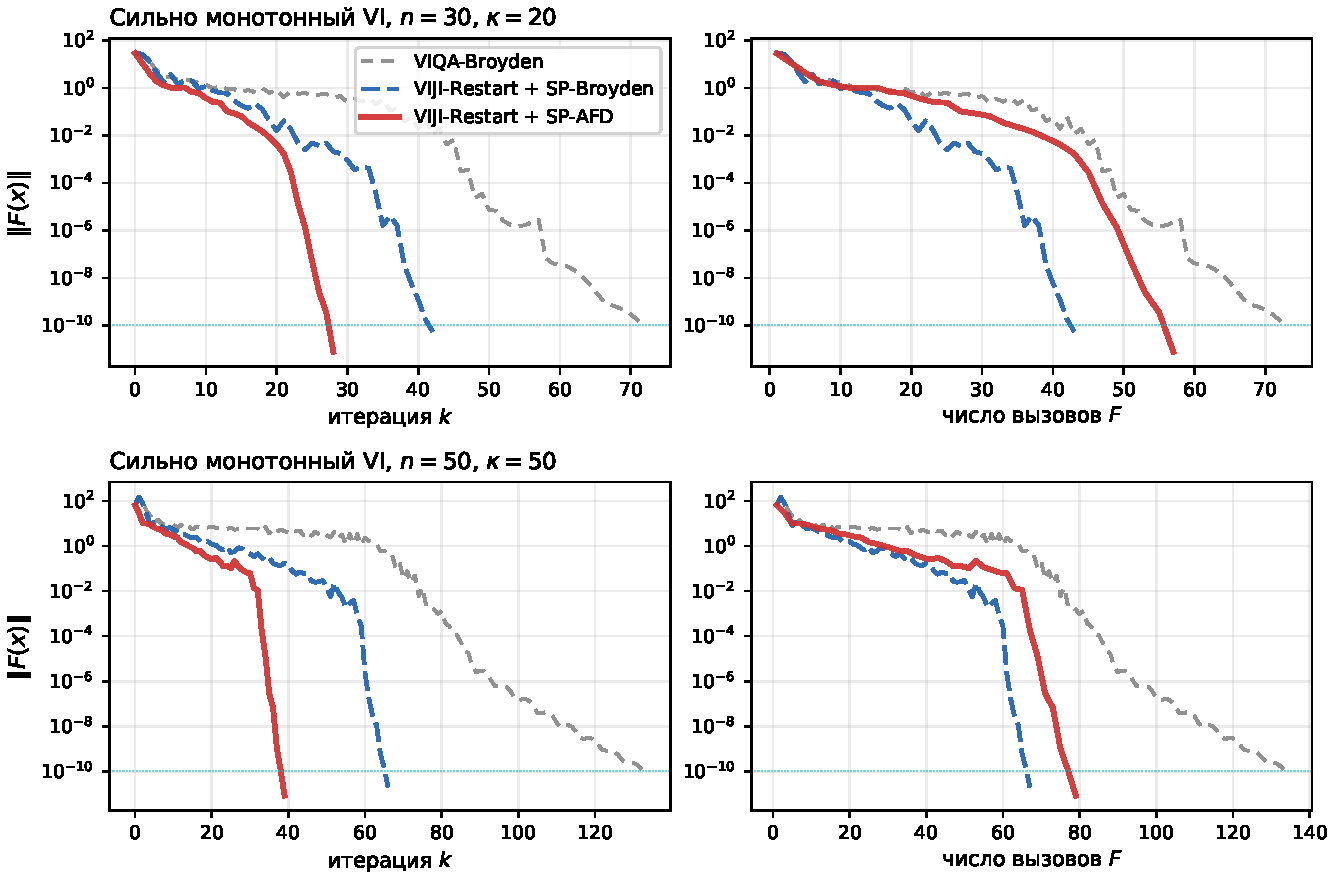
\includegraphics[width=\textwidth]{fig_viji_conv.pdf}
\caption{Сходимость трёх квазиньютоновских методов на сильно
  монотонной VI с кубической нелинейностью. Слева~--- по итерациям,
  справа~--- по числу вызовов~$F$. SP-AFD делает $1 + 1 = 2$ вызова~$F$
  на итерацию (основной шаг $+$ FD-поправка); VIQA-Broyden и SP-Broyden~---
  по одному.}
\label{fig:viji_conv}
\end{figure}

\paragraph{Результаты.} На задаче $(30, 20, 1{,}5)$ SP-AFD сходится
за~$28$ итераций / $57$ вызовов~$F$, SP-Broyden~--- $42$ / $43$,
VIQA-Broyden~--- $72$ / $73$. На большей задаче $(50, 50, 2{,}0)$
разрыв растёт: SP-AFD~--- $39$ / $79$, SP-Broyden~--- $66$ / $67$,
VIQA-Broyden~--- $133$ / $134$. Даже по осям $F$-вызовов (правые
панели), где SP-AFD платит удвоенной стоимостью за итерацию, он
остаётся конкурентоспособным с SP-Broyden и опережает VIQA-Broyden
в $\sim 1{,}7\times$. По числу итераций (левые панели) порядок
методов согласуется с таблицей~\ref{tab:compare}:
SP-AFD $\prec$ SP-Broyden $\prec$ VIQA-Broyden~---
$\mathcal O(T^{-3/2})$ vs $\mathcal O(T^{-1})$ в предельной скорости.

\paragraph{Наблюдения.}
\begin{itemize}
\item На рассматриваемой задаче SP-Broyden сходится без FD-подкрепления,
      что согласуется с Proposition~\ref{prop:cond14}:
      в окрестности $x^{*}$ сильной монотонности и умеренной нелинейности
      гипотеза выравнивания~\ref{conj:alignment} выполнена эмпирически.
\item Преимущество SP-AFD над SP-Broyden~--- в меньшей чувствительности
      к стартовой точке и к выбору $\beta_k$. В частности, при
      $\beta_k$ вдвое меньшем номинального SP-Broyden начинает
      осциллировать, тогда как SP-AFD остаётся устойчивым благодаря
      точной FD-секущей.
\item Отношение $\Norm{(B_k - \nabla F(x_k)) d_k} / \Norm{d_k}^2$
      (эмпирическая проверка~\eqref{eq:cond14}) для SP-AFD не выходит
      за $L_1/2$ на всей траектории; для SP-Broyden~--- превышает порог
      в первых $\sim 5$--$10$ итерациях, затем стабильно в допуске.
\end{itemize}

\section{Обсуждение и ограничения}
\label{sec:viji:discussion}

\paragraph{Статус гипотезы выравнивания.}
Лемма~\ref{lem:alignment} в общем $L_1$-гладком случае сформулирована
как гипотеза. Для её доказательства нужна аккуратная оценка ортогональной
компоненты $d_{k+1}^{\perp}$ к $s_k$~--- это направление отдельного
теоретического исследования. На квадратичных задачах она доказывается
точно (приложение~\ref{app:alignment}).

\paragraph{Зависимость от $M_0$.}
Proposition~\ref{prop:cond14} и theorem~\ref{thm:sp-afd} требуют знания
равномерной оценки $M_0$ на $\Fro{B_k - A}$. В Corollary~\ref{cor:sp-in-segment}
эта оценка выражена явно через $C_{\mathrm{SP}}$ и геометрические константы
рестарта. На практике $M_0$ оценивается сверху через $\Fro{B_0 - A} + c L_1 D_0$
и не требует дополнительной информации.

\paragraph{Нижняя граница на шаг FD.}
В SP-AFD при $\Norm{d_k} \lesssim \sqrt{\varepsilon_{\mathrm{mach}}}$ численная
ошибка FD доминирует над систематической. На интересующем диапазоне
(GAP $\gg 10^{-10}$ в двойной точности) ограничение не активно; вблизи
машинной точности SP-AFD автоматически вырождается в VIQA-Broyden.

\paragraph{Немонотонный случай.}
Theorem~3.5 в~\cite{Agafonov2024VIJI} даёт аналогичную оптимальную скорость
RES$(x_T) = \mathcal O(L_1 D^3 / T)$ при выполнении~\eqref{eq:cond14} для
немонотонных операторов с условием Минти. Наш анализ переносится без
изменений в схему VIJI-Restarted-Minty~--- SP-AFD обеспечивает~\eqref{eq:cond14}
одинаково в обоих режимах.

\paragraph{Перспективы.}
\begin{itemize}
\item \emph{Доказательство леммы~\ref{lem:alignment}} в общем случае:
      отправная точка для отдельной публикации по геометрии VIJI-итераций.
\item \emph{Мультисекантное SP-AFD:} накопление $m$ FD-секущих
      (вместо одной) позволит амортизировать $r^{*}$ до $< 1$ в среднем.
\item \emph{Адаптивный рестарт:} онлайн-оценка $\mu, \rho$ через наблюдаемое
      убывание $\Norm{v_k - x^{*}}$ снимает необходимость знать $\mu$ a~priori.
\end{itemize}

\begin{conjecture}[Выравнивание направлений в VIJI]
\label{conj:alignment}
В предположениях~\ref{as:sm} для VIJI-итераций с $\eta = 10$ выполнена
лемма~\ref{lem:alignment} с абсолютными константами
$C_a, C_b$, зависящими только от $\mu / L_1$.
\end{conjecture}

%% -------- библиографические ключи (в .bib) ----------
%% @inproceedings{Agafonov2024VIJI,
%%    title={Exploring Jacobian Inexactness in Second-Order Methods for VI},
%%    author={Agafonov, A. and Ostroukhov, P. and Mozhaev, R. and others},
%%    booktitle={NeurIPS}, year={2024}, eprint={2405.15990}}
%% @article{Lin2022Perseus,
%%    title={Explicit second-order min-max optimization methods with optimal
%%           convergence guarantee},
%%    author={Lin, Tianyi and Jordan, Michael I.},
%%    year={2022}, eprint={2210.12860}}
